\documentclass[a4paper,10pt,notitlepage]{article}
\usepackage{ctex,geometry,graphicx,tikz,setspace,paralist,fancyhdr,caption}
\geometry{
	left=1.5cm,
	right=1.5cm,
	top=1.4cm,
	bottom=2cm,}
\newcommand{\rec}{
	\begin{tikzpicture}[remember picture,overlay]
		% 绘制边框
		\draw[line width=1.2pt] ([xshift=0.5cm,yshift=0.5cm] current page.south west) rectangle ([xshift=-0.5cm,yshift=-0.8cm] current page.north east);
	\end{tikzpicture}
	
}
\pagestyle{fancy}
\fancyhf{}
\fancyhead[C]{\rec}  % 在页眉中绘制图形
\fancyhead[L]{模电实验报告}
\fancyhead[R]{实验八 \quad 波形发生电路}
\fancyfoot[C]{\thepage}
\begin{document}
	\large
	\onehalfspacing
	\begin{figure}[h]
		\raggedright
		
\includegraphics{预习报告/1.png}
	\end{figure}
	\centering
	{\Huge\textbf{模电实验报告}\par}
	\vspace{0.2cm}
	{\huge{实验内容:波形发生电路}\par}
	\raggedright
	\vspace{0.3cm}
	\begin{centering}
		{\large 院系:电子与信息工程学院\hfill 学号:22309080\hfill 审批:\hspace{2cm} \par
			专业:通信工程\hfill 实验人:梁倍铭\hfill 日期:2023年12月01日 \par}
	\end{centering}
	\vspace{0.3cm}
	\section*{一、实验目的}
	\begin{enumerate}
		\item 掌握波形发生电路的特点和分析方法。
		\item 熟悉波形发生器设计方法。
	\end{enumerate}
	\section*{二、原理简介}
	\begin{enumerate}
		\item 方波发生电路\par 
		实验电路如图8-1 所示。\par 
		\begin{figure}[h]
			\centering
			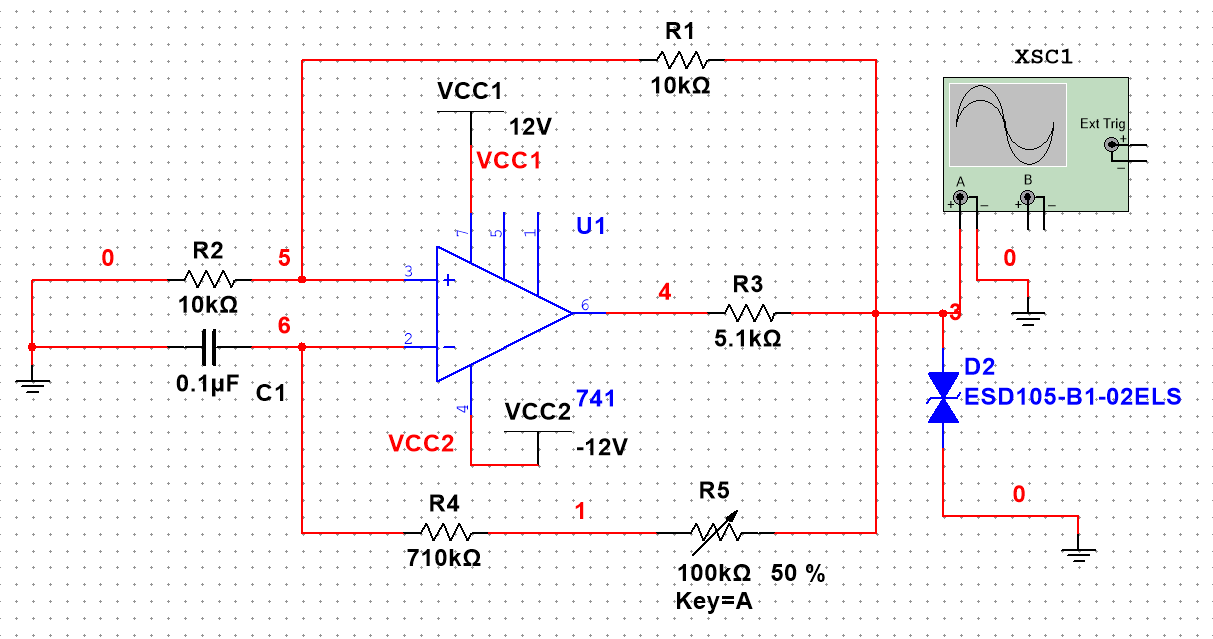
\includegraphics[width=0.5\textwidth]{1.png}
			\caption*{图8-1 方波发生电路}
		\end{figure}
		\qquad 图8-1 所示的方波发生电路由反向输入的滞回比较器(即施密特触发器)和RC 回
		路组成,滞回比较器引入正反馈,RC 回路既作为延迟环节,又作为负反馈网络,电路通过
		RC 充放电来实现输出状态的自动转换。\par 
		分析电路,可知道滞回比较器的门限电压 $\pm U_T=\pm \frac{R_1}{R_1+R_2}U_Z$。\par 
		\qquad 当$U_O$输出为$U_Z$时,$U_O$通过R对C充电,直到C上的电压$U_C$上升到门限电压$U_T$,
		此时输出$U_O$反转为$-U_Z$,电容C通过R放电,当C上的电压$U_C$下降到门限电压$-U_T$,
		输出$U_O$再次反转为$U_Z$,此过程周而复始,因而输出方波。根据分析充放电过程可得公
		如下:
		$$T=2RC\ln{(1+\frac{2R_1}{R_2})},f=\frac{1}{T},(R1=3R_{12},R_2=3R_5,R_1=R_2=10k,C=0.1\mu)$$
		\item 占空比可调的矩形波发生电路\par 
		实验电路如图8-2 所示。\par 
		\begin{figure}[h]
			\centering
			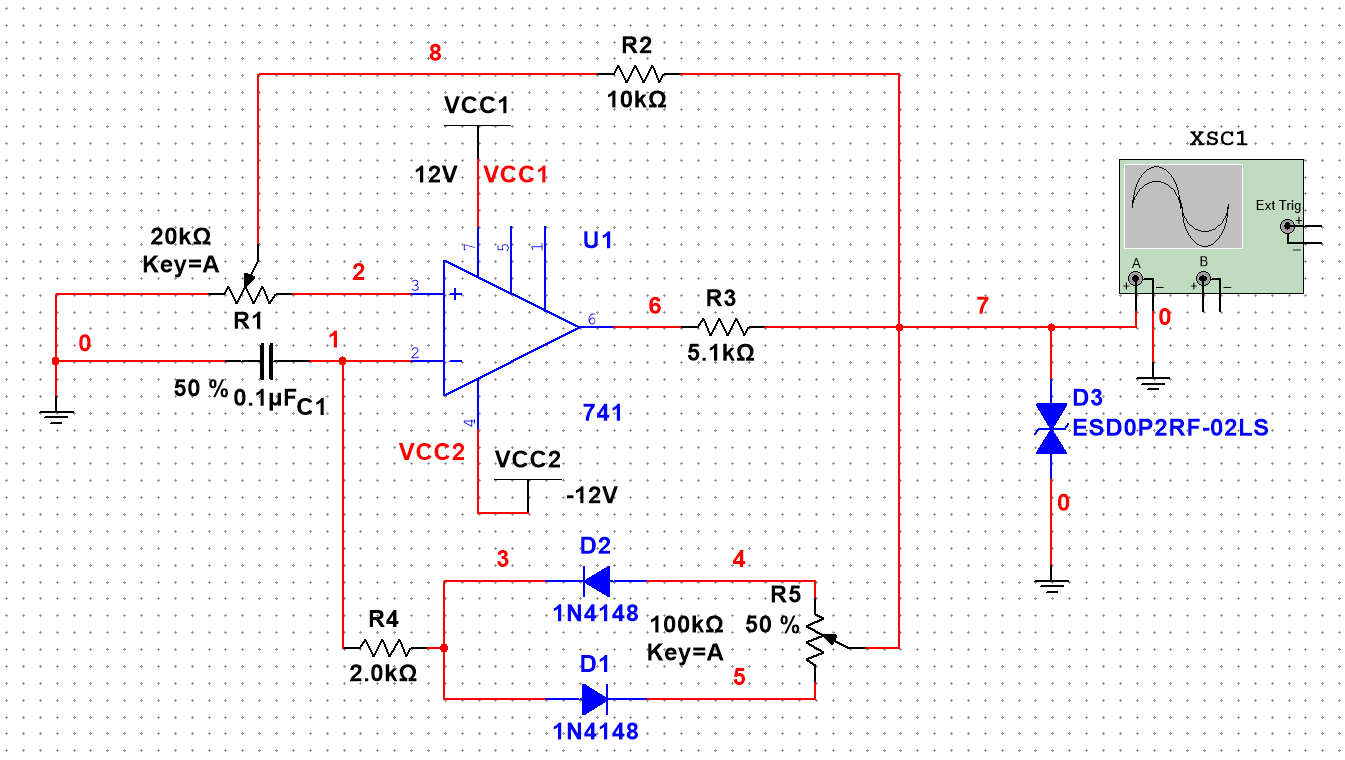
\includegraphics[width=0.5\textwidth]{2.png}
			\caption*{图8-2 占空比可调的矩形波发生电路}
		\end{figure}
		\qquad 图8-2 原理与图8-1 相同,但由于两个单向导通二级管的存在,其充电回路和放电
		回路的电阻不同,设电位器$R_{p1}$中属于充电回路部分(即$R_{p1}$上半)的电阻为${R}'$,电位器
		$R_{p1}$中属于放电回路部分(即$R_{p1}$下半)的电阻为${R}''$,如不考虑二极管单向导通电压可得公式:
		$$T=t_1+t_2=(2R+{R}'+{R}'')C\ln{(1+\frac{2R_{p2}}{R_2})},f=\frac{1}{T}$$
		占空比$$q=\frac{R+{R}'}{2R+{R}'+{R}''},$$
		调节$R_{p2}=10k\Omega$,由各条件可计算出$f\approx 87.54Hz$。之所以与理论计算值有相当大的
		差异,是因为理论计算时忽略了二极管正向导通电压0.7 伏的关系,实际充放电电流比理
		论小,所以频率要比理论低。
		\item 三角波发生电路\par 
		实验电路如图8-3 所示。\par 
		\begin{figure}[h]
			\centering
			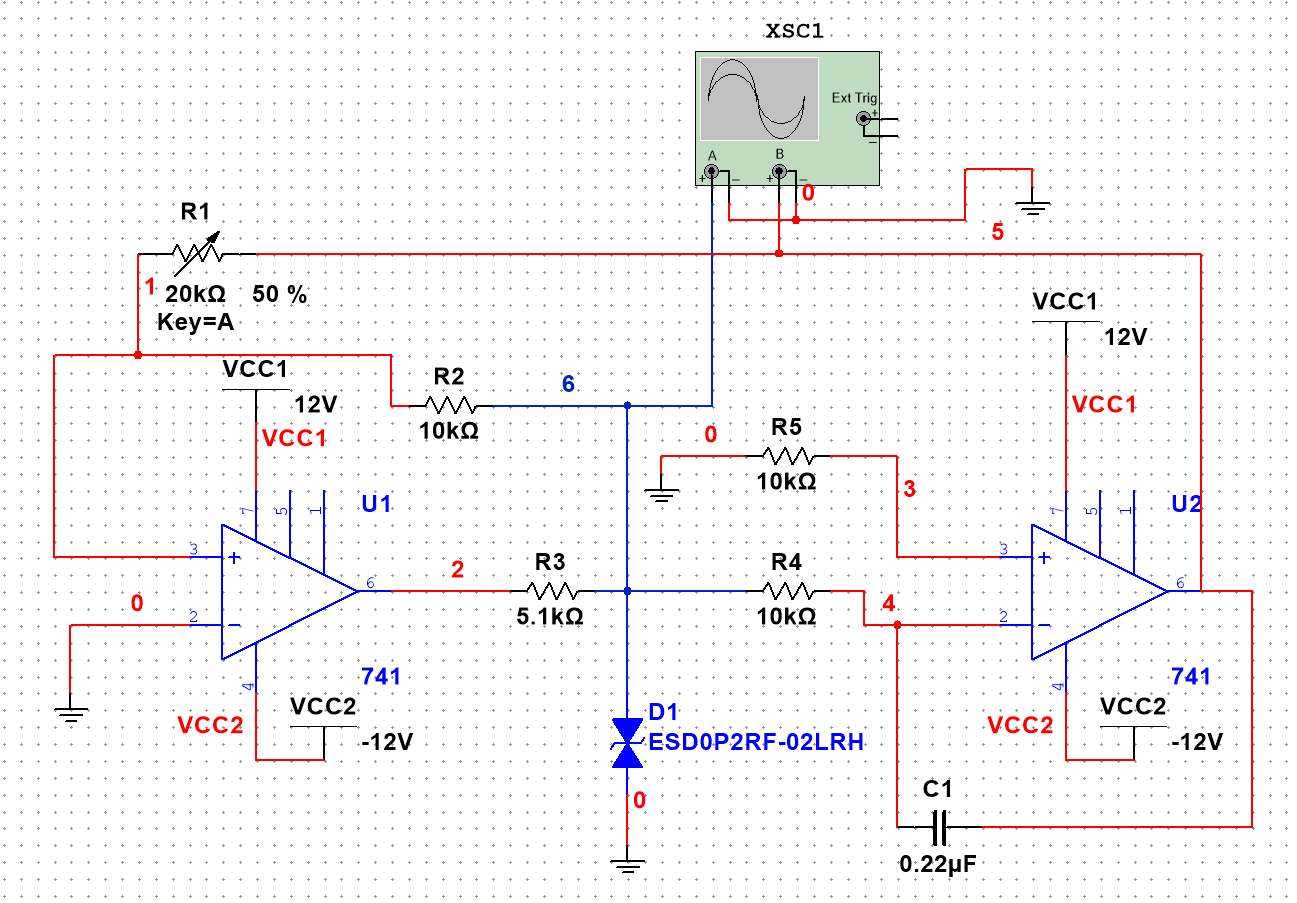
\includegraphics[width=0.5\textwidth]{3.png}
			\caption*{图8-3 三角波发生电路}
		\end{figure}
		\qquad 三角波发生电路是用正相输入滞回比较器与积分电路组成,与前面电路相比较,积分
		电路代替了一阶RC 电路用作恒流充放电电路,从而形成线性三角波,同时易于带负载。
		分析滞回比较器,可得$\pm U_T=\pm \frac{R_P}{R_1}U_Z,$
		分析积分电路,有$$U_{O2}=-\frac{1}{R_3C}\int U_{O1}\mathrm{d}t,$$
		所以有$$\frac{U_Z}{R_3C}\cdot \frac{T}{2}=U_T-(-U_T)=2\frac{R_P}{R_1}U_Z,$$
		所以$$T=4\frac{R_P}{R_1}R_3C,f=\frac{1}{T},U_{O2m}=U_T$$
		选$R_1=3R_5=10K,R_3=3R_{14}=10K,R_P=10K\Omega$,计算得$f=113.6Hz$。
		\item 锯齿波发生电路\par 
		实验电路如图8-4 所示。\par
		\begin{figure}[h]
			\centering
			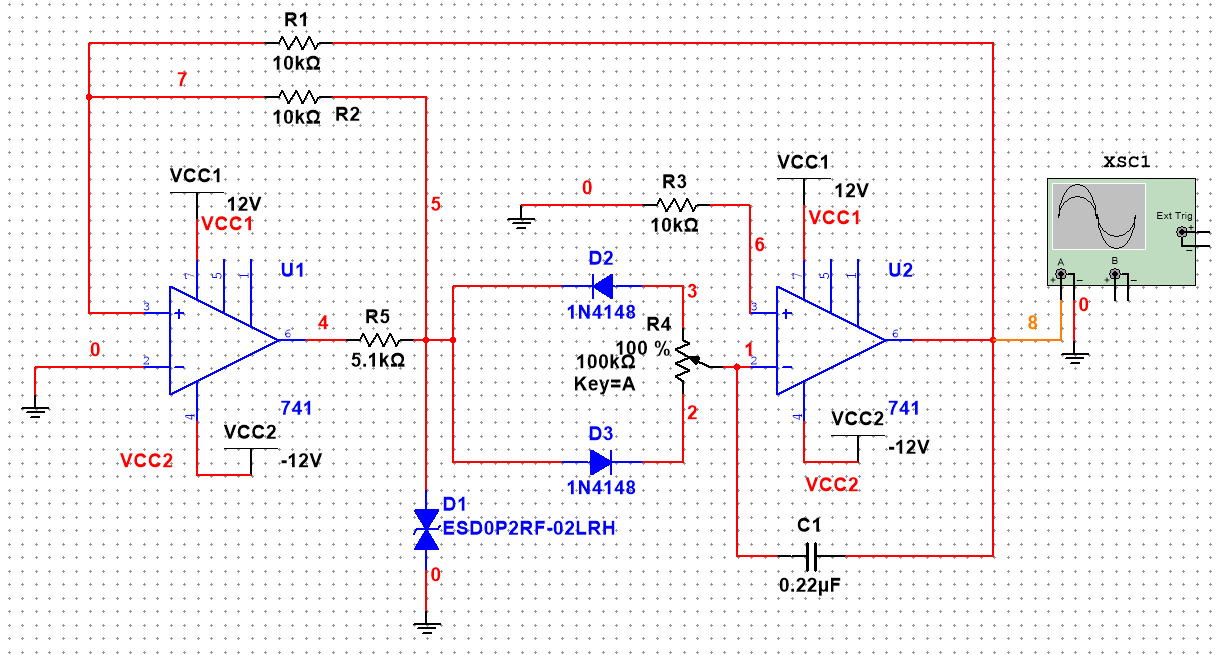
\includegraphics[width=0.5\textwidth]{4.png}
			\caption*{图8-4 锯齿波发生电路}
		\end{figure}
		\qquad 电路分析与前面一样,$\pm U_T=\pm \frac{R_1}{R_2}U_Z$,设当
		$U_{O2}=U_Z$时,积分回路电阻(电位
		器上半部分)为${R}'$,当$U_{O2}=-U_Z$时,积分回路电阻(电位器下半部分)为${R}''$。考虑
		到二极管的导通压降可得:
		$$t_1=\frac{2\frac{R_1}{R_2}U_Z}{U_Z-0.7}{R}'C,t_2=\frac{2\frac{R_1}{R_2}U_Z}{U_Z}{R}''C,T=t_1+t_2,f=\frac{1}{T},$$
		占空比$$q=\frac{t_1}{t_2}=\frac{{R}'}{{R}'+{R}''}$$
	\end{enumerate}
	\section*{三、实验内容和步骤}
	\begin{enumerate}
		\item 方波发生电路
		\begin{enumerate}
			\item 按电路图8-1 接线,观察Vo 波形及频率,与预习比较。\par 
			仿真波形和实验波形图如图8-5和图8-6
			\begin{figure}
				\centering
				\begin{minipage}{0.3\textwidth}
					\centering
					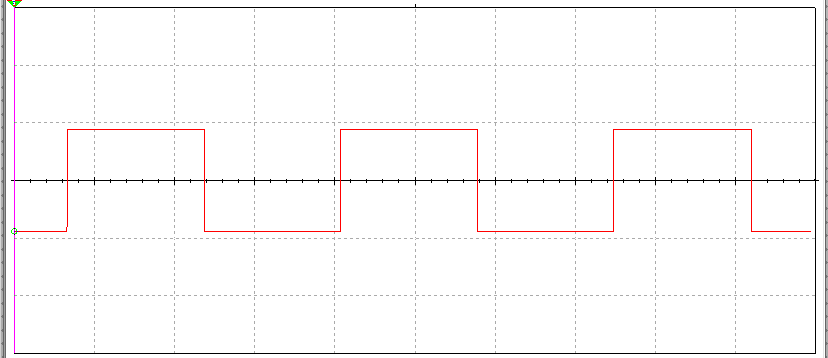
\includegraphics[width=\textwidth]{预习报告/2.png}
					\caption*{图8-5 仿真方波波形}
				\end{minipage}
				\qquad
				\begin{minipage}{0.3\textwidth}
					\centering
					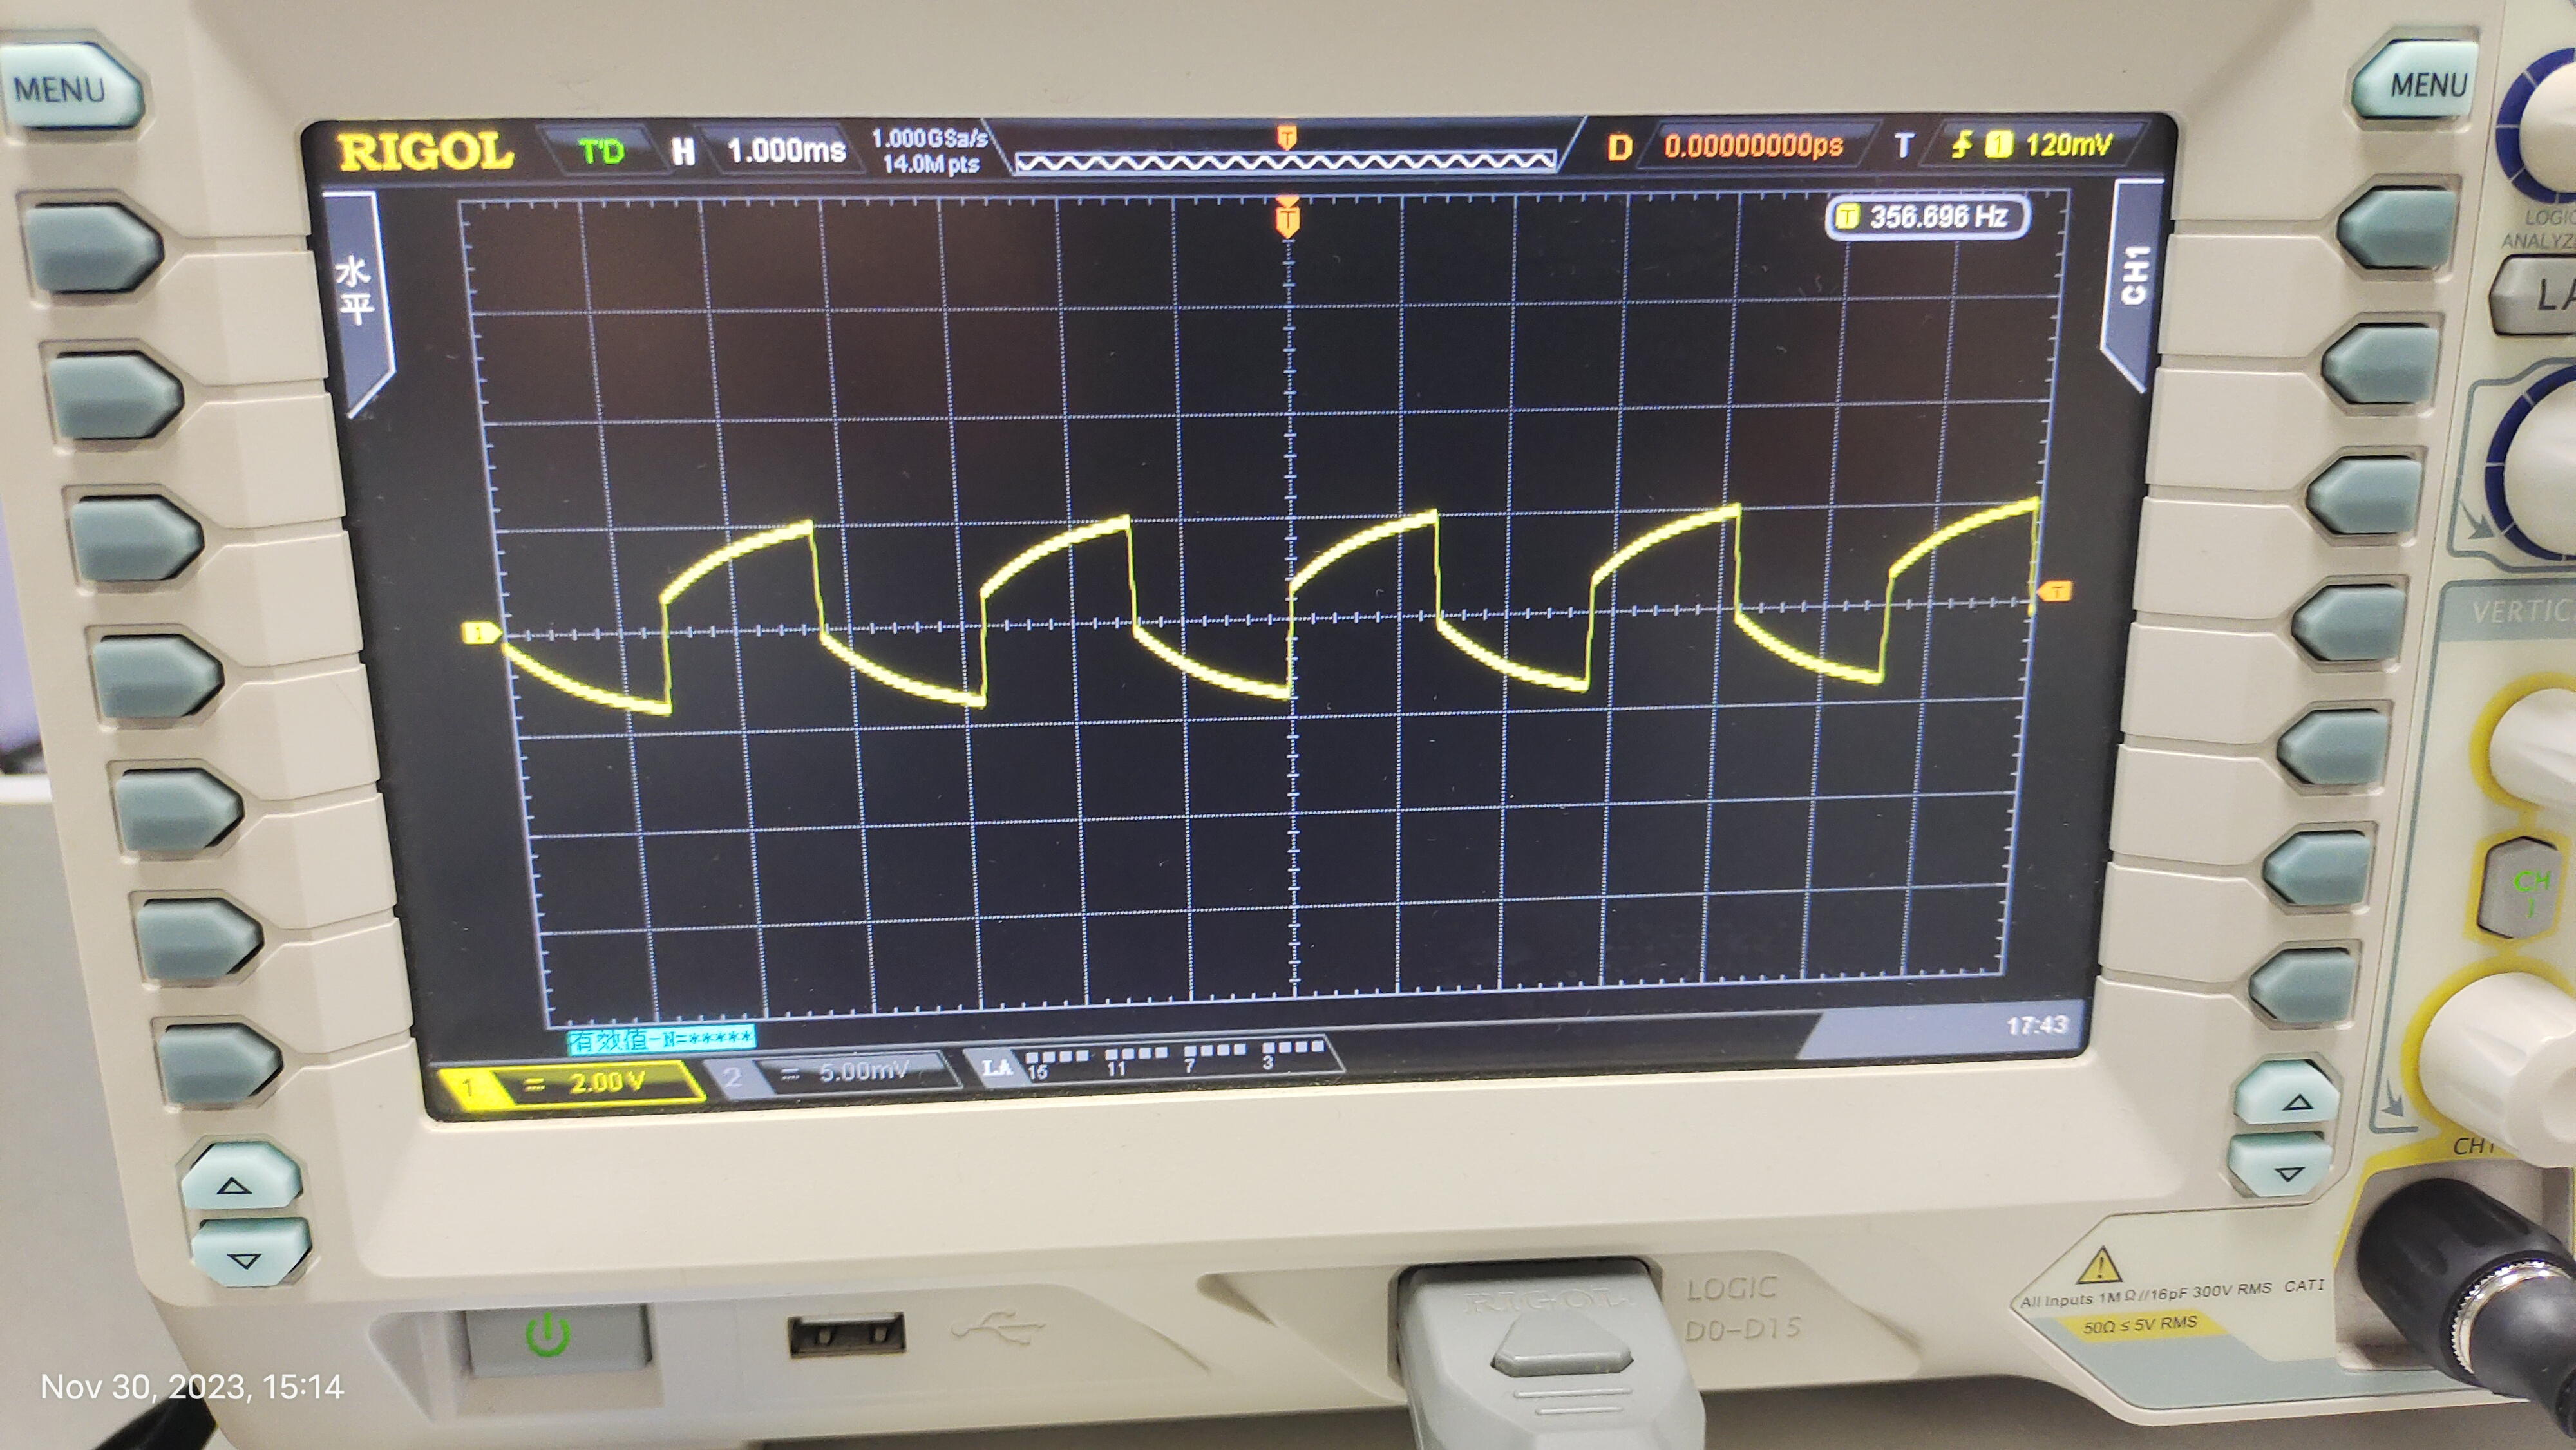
\includegraphics[width=\textwidth]{1.jpg}
					\caption*{图8-6 实验方波波形}
				\end{minipage}
			\end{figure}
			\item 分别测出R= l0K,110K 时的频率,输出幅值,与预习比较。\par 
			频率和幅值如表8-1和表8-2所示
			\begin{figure}
				\centering
				\begin{minipage}{0.3\textwidth}
					\centering
					\begin{tabular}{|c|c|c|}
						\hline
						& 频率(Hz) & 幅值(V) \\
						\hline
						仿真 & 388.8 & 6.47 \\
						\hline 
						实验 & 358.4 & 1.26  \\
						\hline
					\end{tabular}
					\caption*{表8-1 10k时的频率与幅值}
				\end{minipage}
				\qquad
				\begin{minipage}{0.3\textwidth}
					\centering
					\begin{tabular}{|c|c|c|}
						\hline
						& 频率(Hz) & 幅值(V) \\
						\hline
						仿真 & 40.66 & 8.55 \\
						\hline 
						实验 & 89.60 & 2.74  \\
						\hline
					\end{tabular}
					\caption*{表8-2 110k时的频率与幅值}
				\end{minipage}
			\end{figure}
			\item 要想获得更低的频率应如何选择电路参数?试利用实验箱上给出的元器件进行条
			件实验并观测之。\par 
			想要获得更低频率增大R即可\par 
			仿真波形如图8-7,实验波形如图8-8
			\begin{figure}
				\centering
				\begin{minipage}{0.3\textwidth}
					\centering
					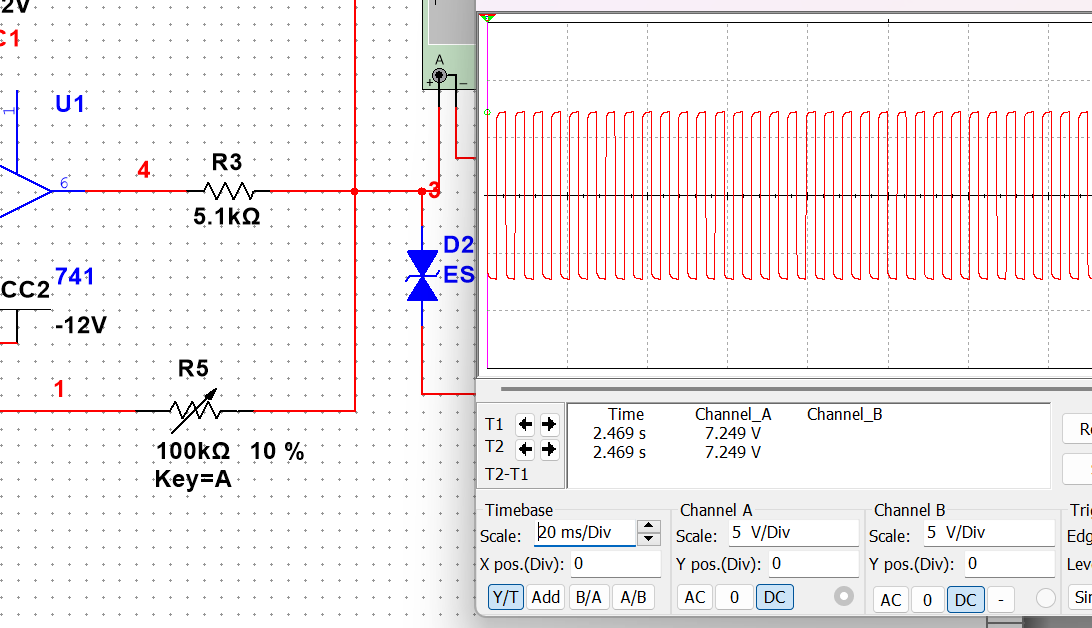
\includegraphics[width=\textwidth]{5.png}
					\caption*{仿真R=20$k\Omega$波形}
				\end{minipage}
				\qquad
				\begin{minipage}{0.3\textwidth}
					\centering
					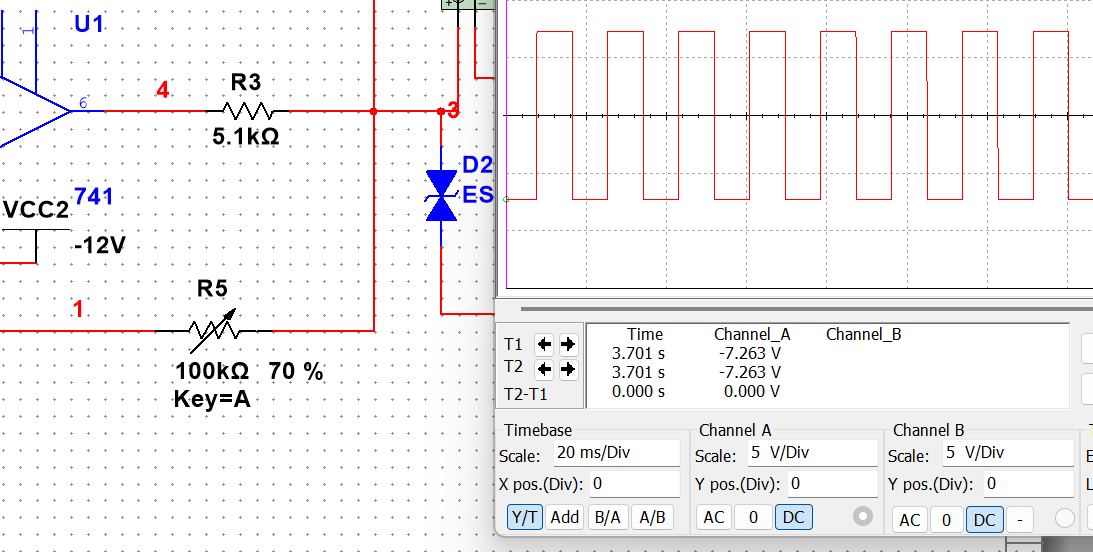
\includegraphics[width=\textwidth]{6.png}
					\caption*{仿真R=80$k\Omega$波形}
				\end{minipage}
				\caption*{图8-7 仿真波形}
			\end{figure}
			\begin{figure}
				\centering
				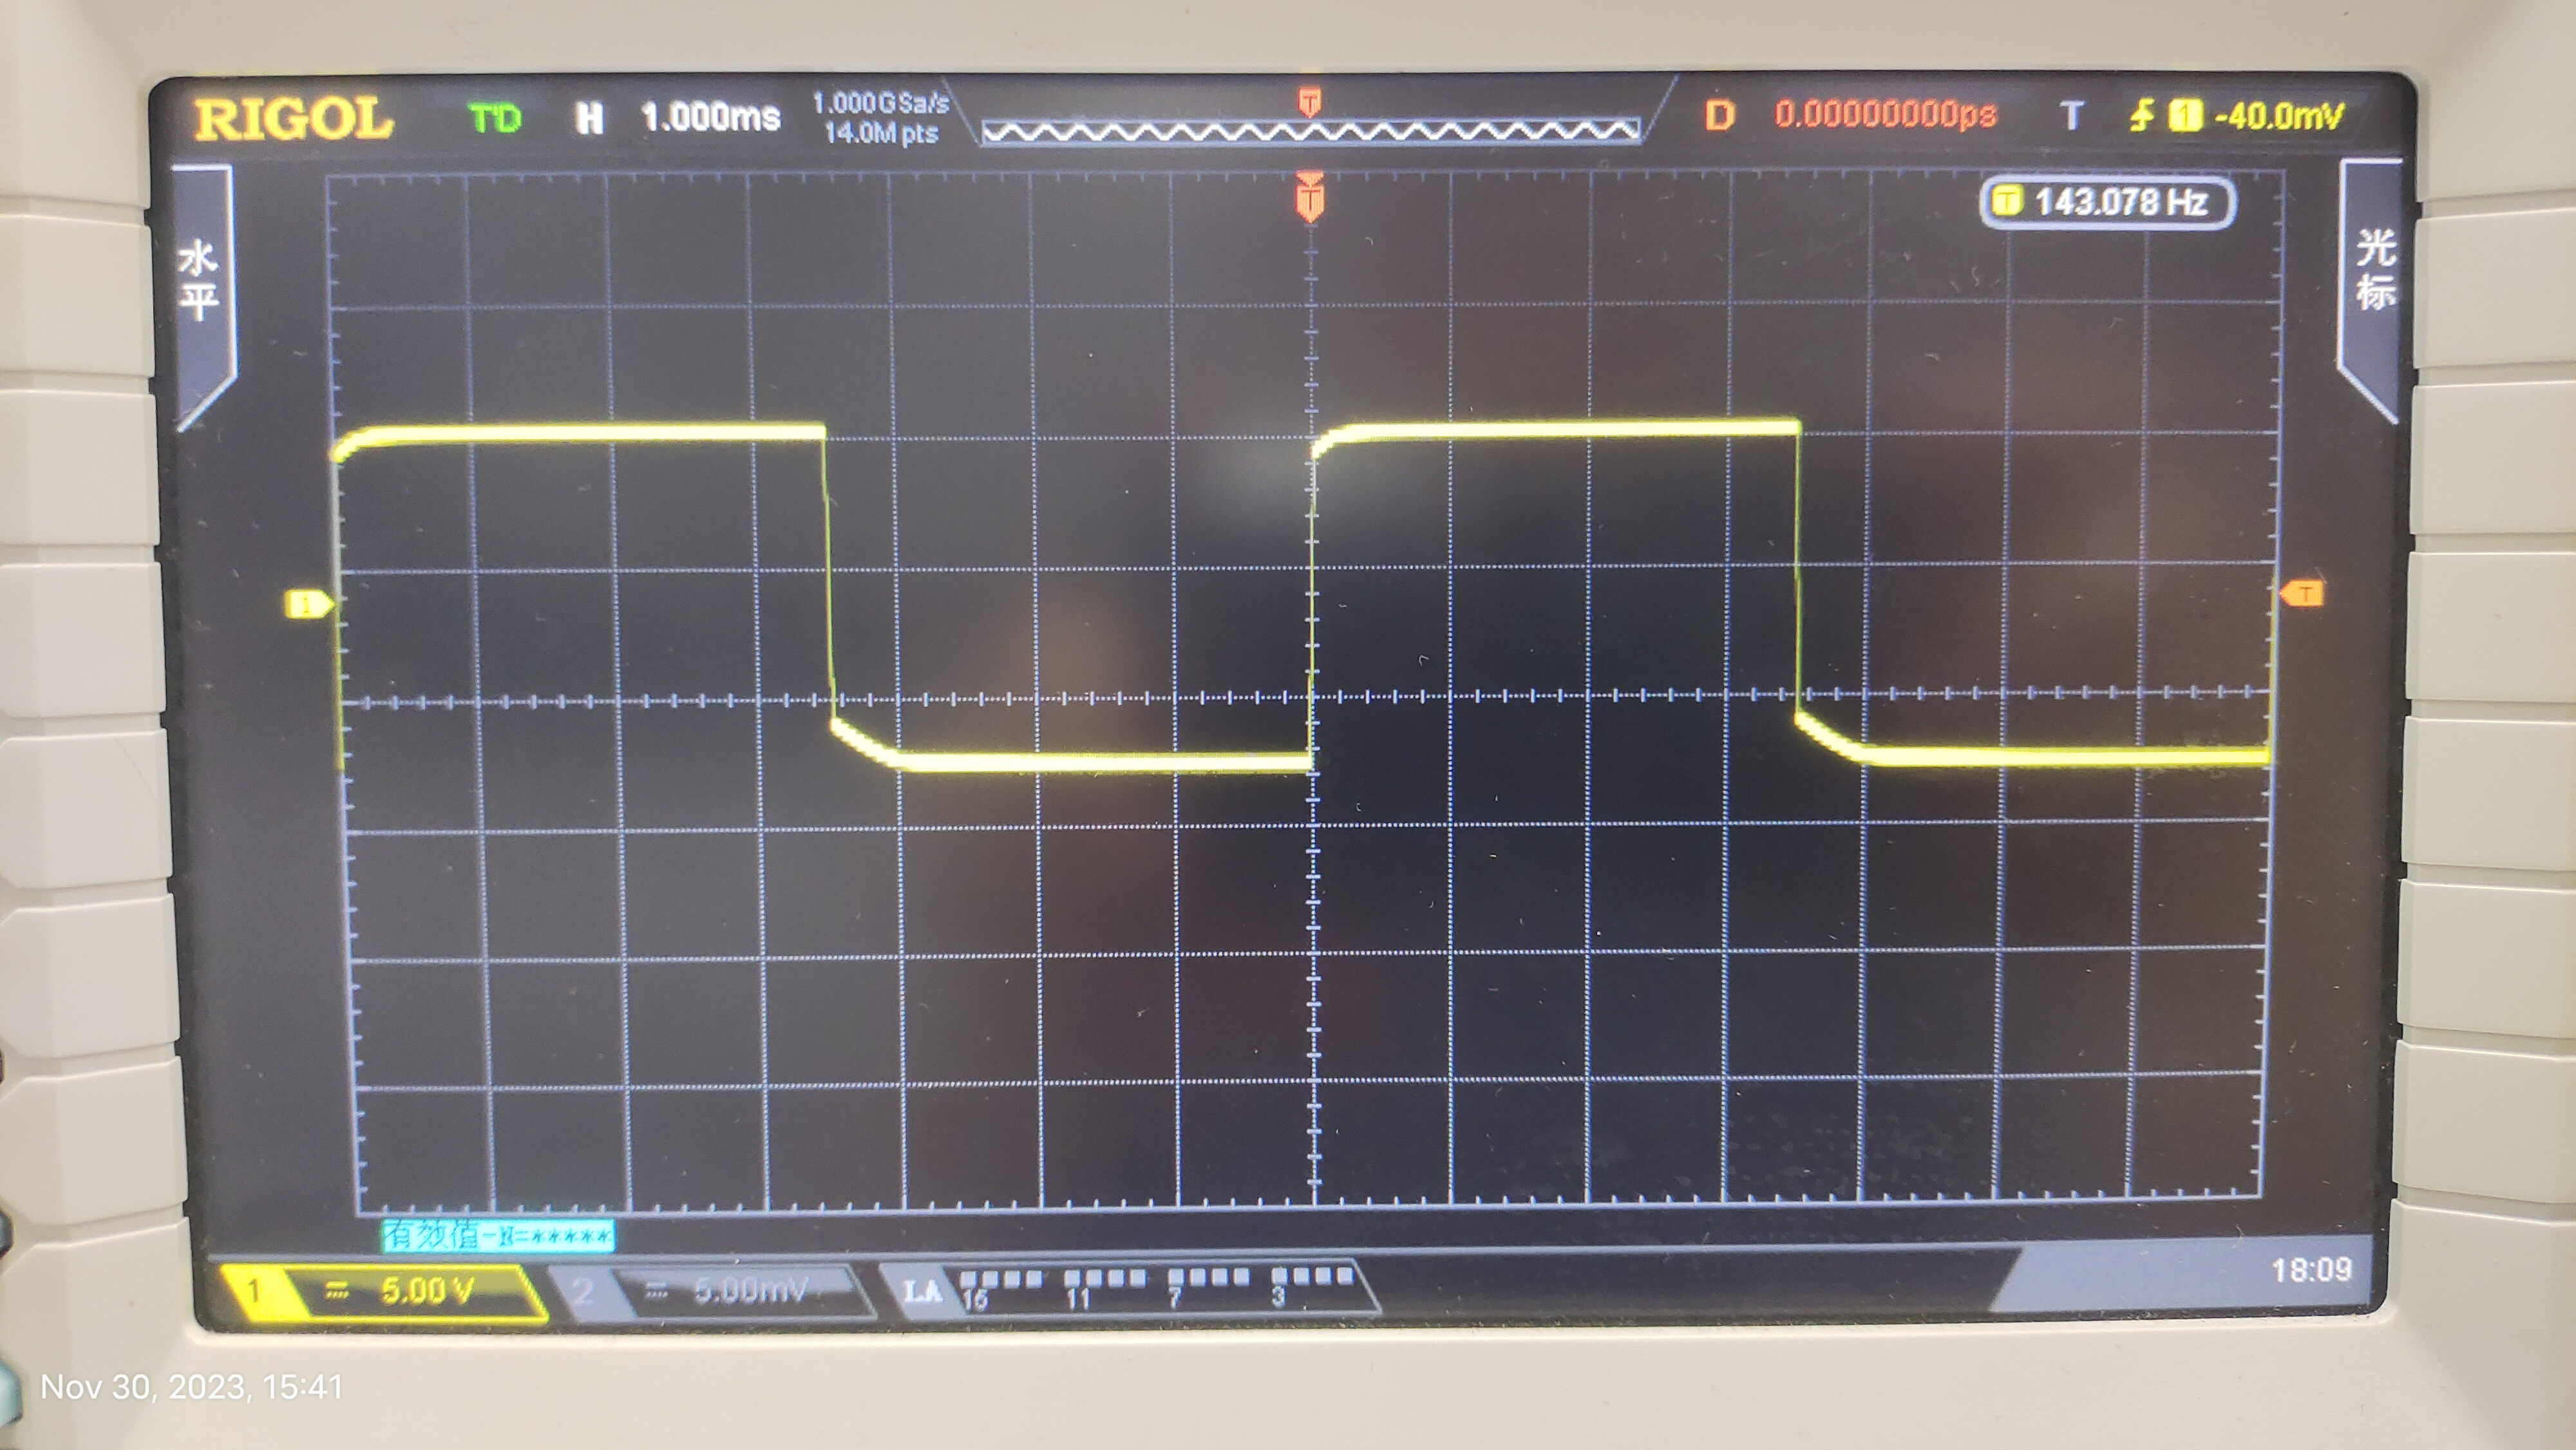
\includegraphics[width=0.4\textwidth]{2.jpg}
				\caption*{图8-8 增大R后的实验波形}
			\end{figure}
		\end{enumerate}
		\newpage
		\item 占空比可调的矩形波发生电路
		\begin{enumerate}
			\item 按图8-2 接线,观察并测量Vo 电路的振荡频率、幅值及占空比。\par 
			仿真波形如图8-9,实验波形如图8-10\par 
			\begin{figure}[h]
				\centering
				\begin{minipage}{0.3\textwidth}
					\centering
					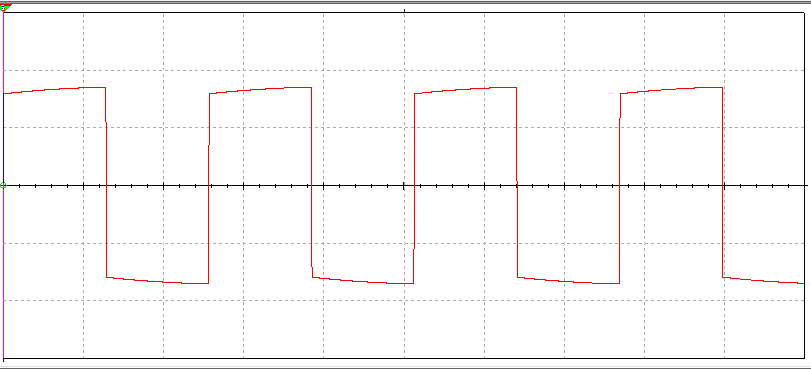
\includegraphics[width=\textwidth]{预习报告/3.png}
					\caption*{图8-9 仿真占空比可调方波波形}
				\end{minipage}
				\qquad
				\begin{minipage}{0.3\textwidth}
					\centering
					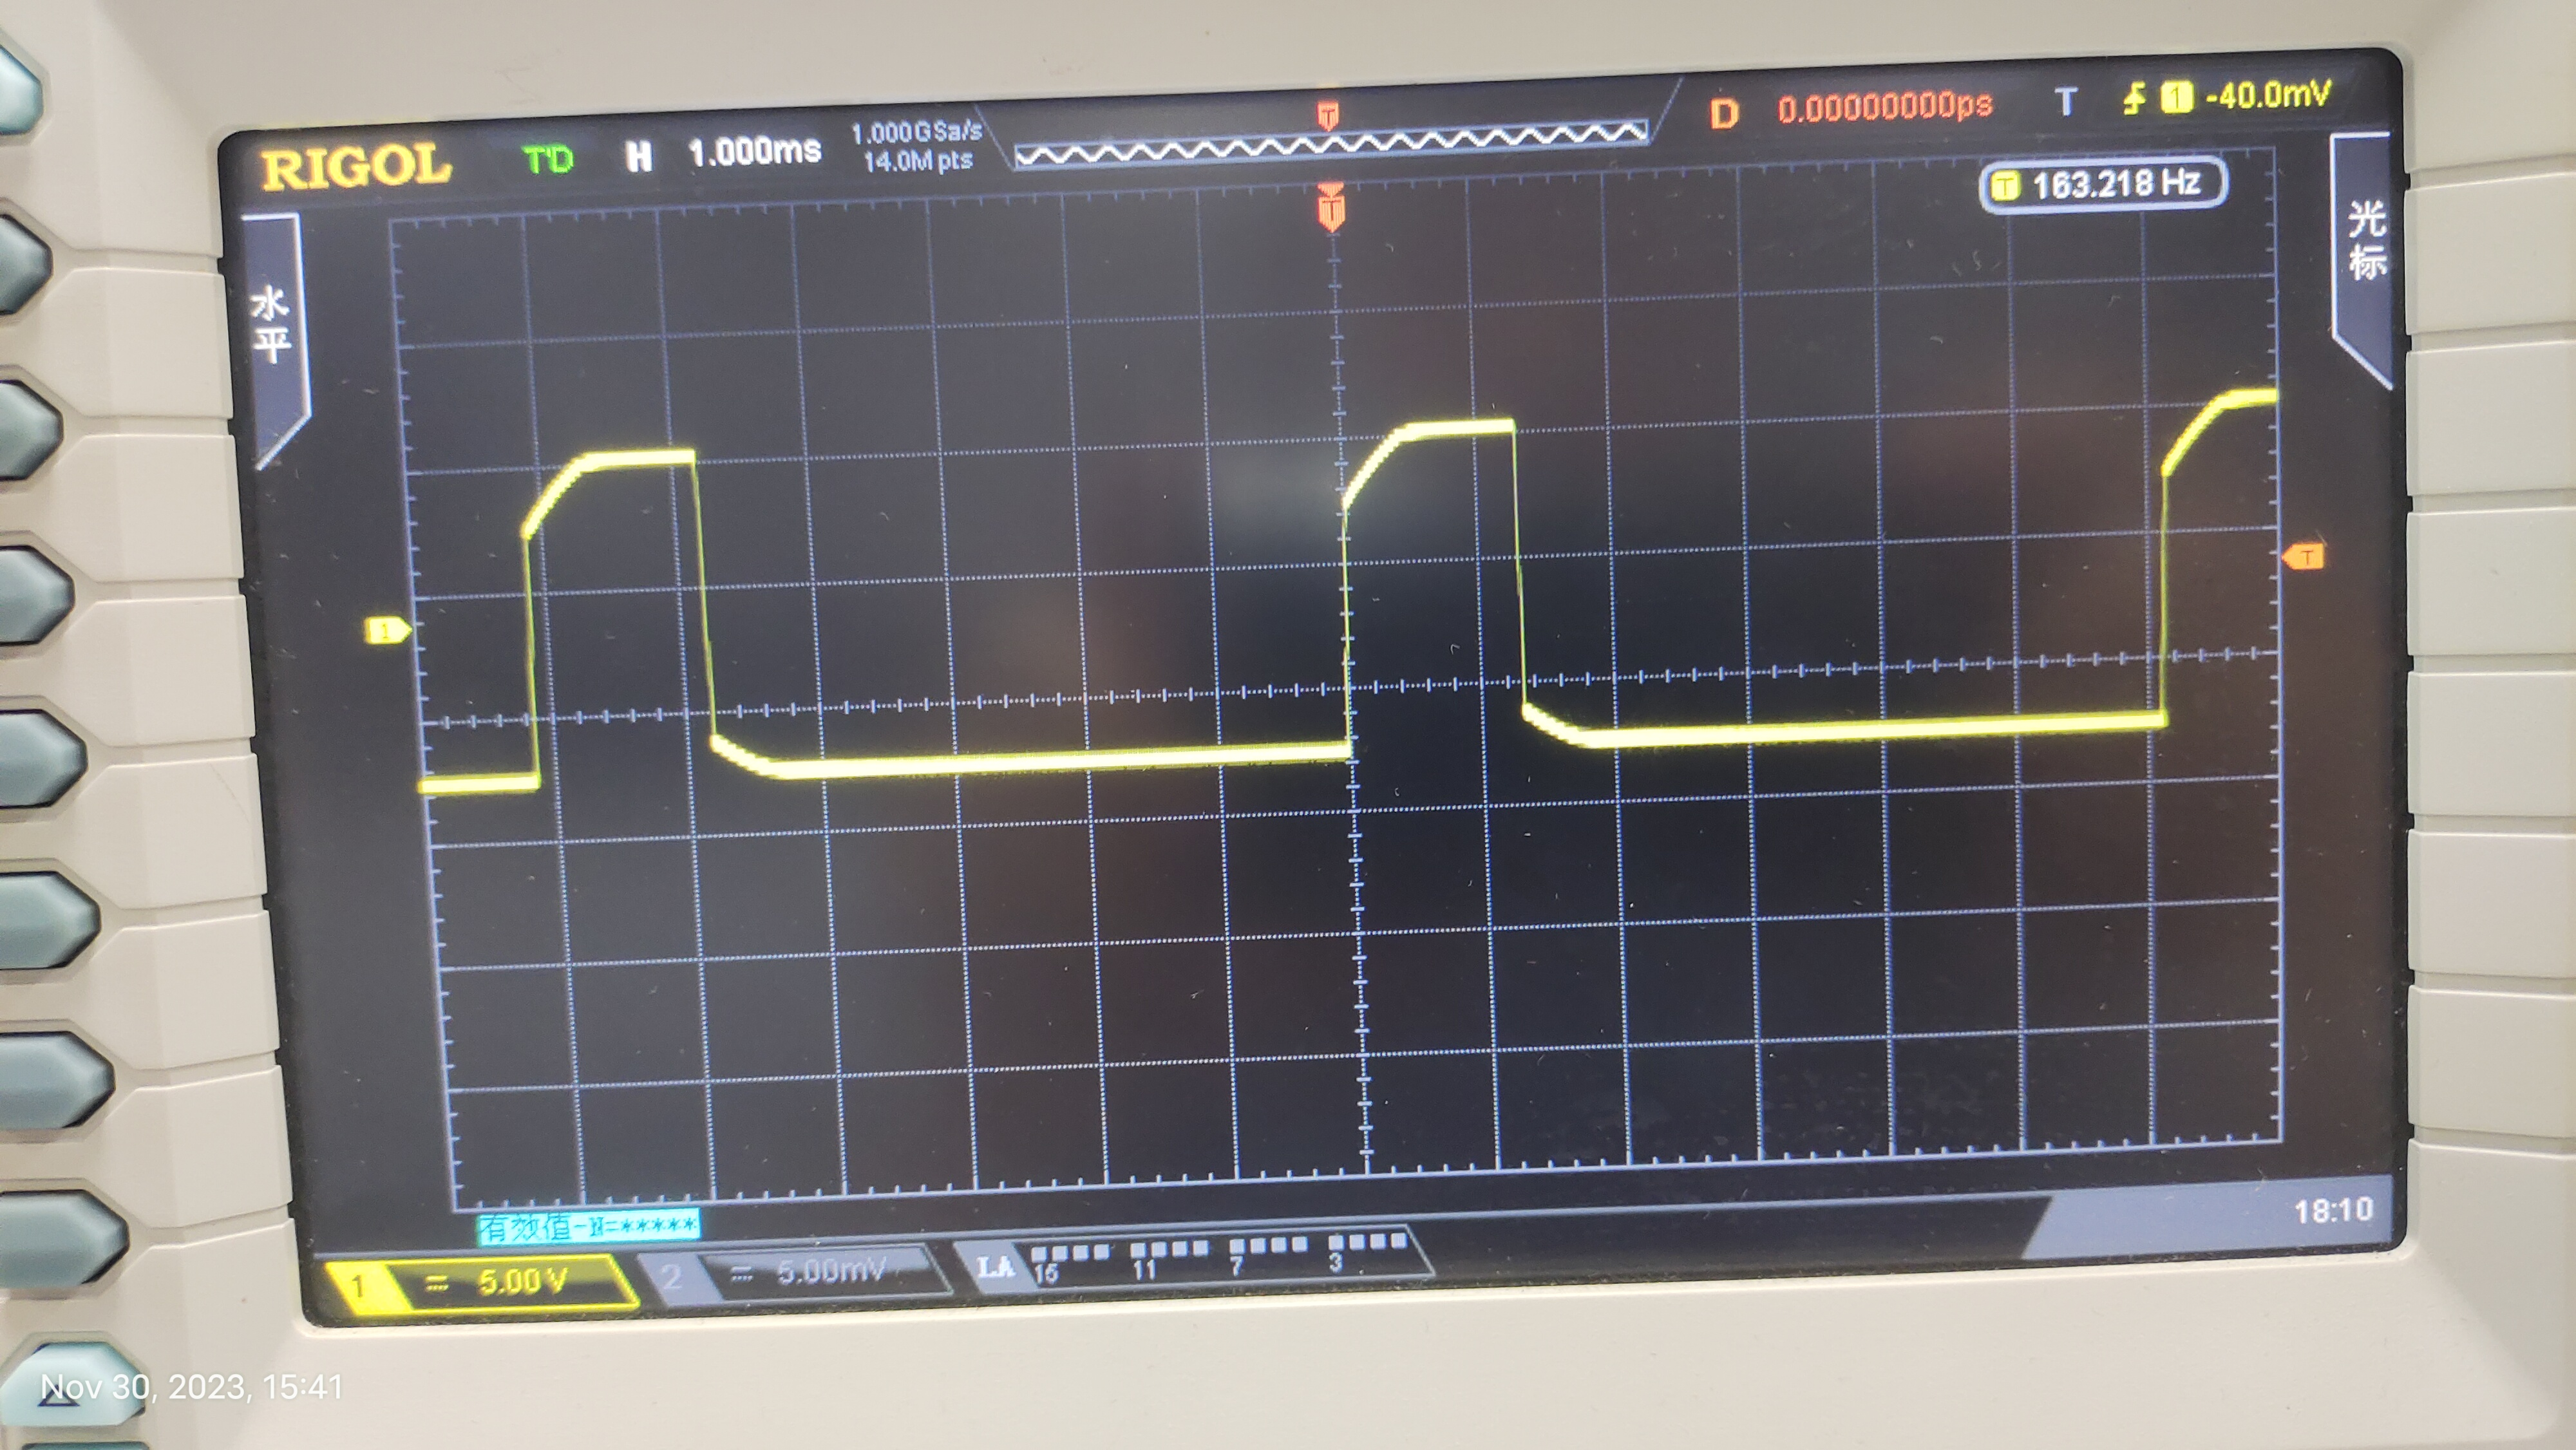
\includegraphics[width=\textwidth]{3.jpg}
					\caption*{图8-10 实验占空比可调方波波形}
				\end{minipage}
			\end{figure}
			对电路振荡频率、幅值及占空比的观测如表8-3
			\begin{table}[h]
				\centering
				\begin{tabular}{|c|c|c|c|}
					\hline
					& 频率(Hz) & 幅值(V) & 占空比(\%) \\
					\hline
					仿真 & 77.52 & 8.348 & 49.3 \\
					\hline 
					实验 & 210.1 & 6.3 & 50 \\
					\hline
				\end{tabular}
				\caption*{表8-3 观测数据}
			\end{table}
			\item 若要使占空比更大,应如何选择电路参数并用实验验证。\par 
			想要波形占空比更大,调节RP1使得正向充电的时间更长即可\par 
			仿真波形如图8-11,实验波形如图8-12
			\begin{figure}[h]
				\centering
				\begin{minipage}{0.3\textwidth}
					\centering
					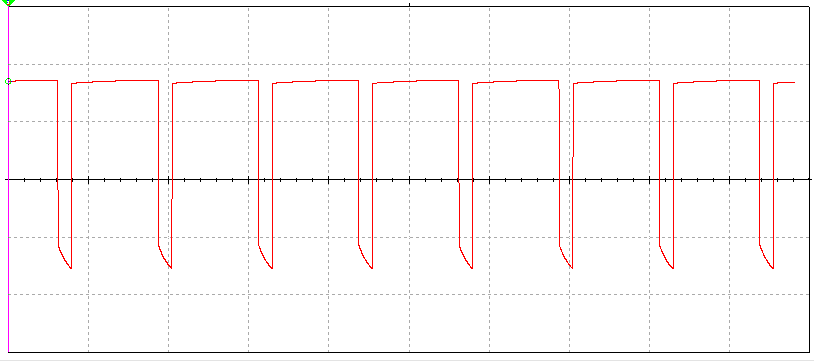
\includegraphics[width=\textwidth]{7.png}
					\caption*{图8-11 增大占空比仿真波形}
				\end{minipage}
				\qquad
				\begin{minipage}{0.3\textwidth}
					\centering
					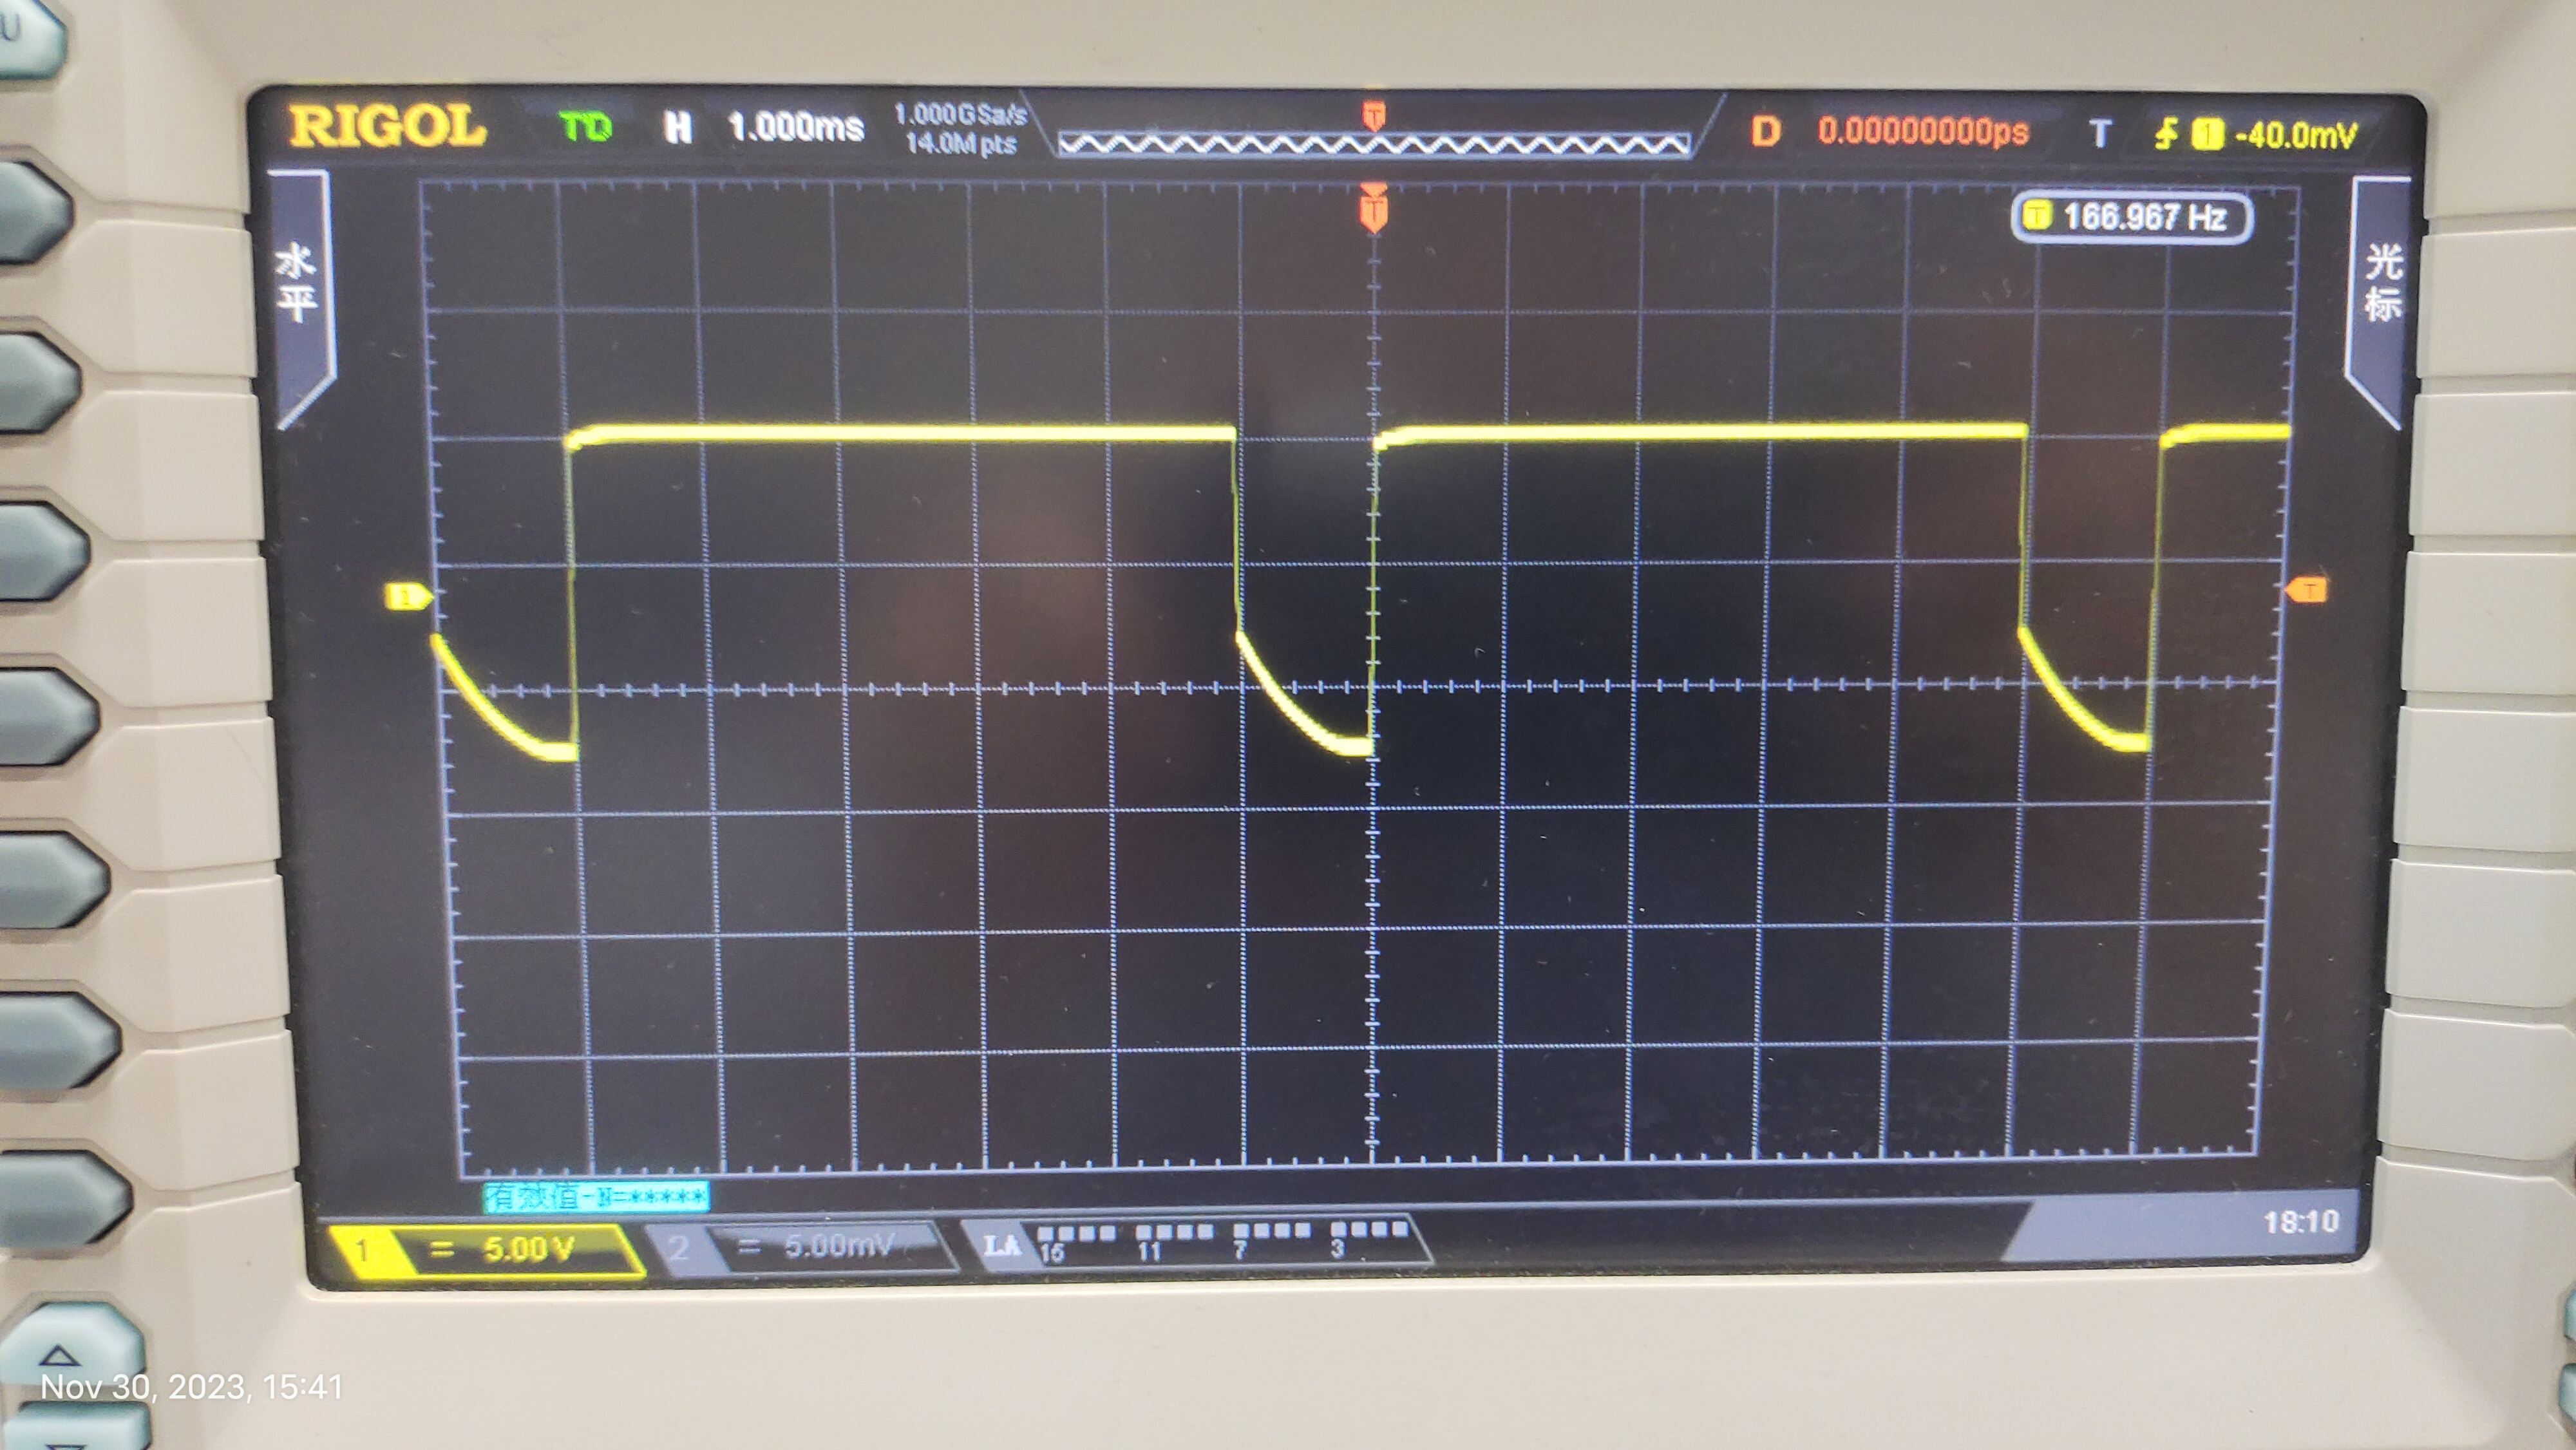
\includegraphics[width=\textwidth]{4.jpg}
					\caption*{图8-12 增大占空比实验波形}
				\end{minipage}
			\end{figure}
		\end{enumerate}
		\item 三角波发生电路
		\begin{enumerate}
			\item 按图8-3 接线,分别观测Vo1 及Vo2 的波形并记录。\par 
			仿真观测结果如图8-13,实验观测结果如图8-14
			\begin{figure}
				\centering
				\begin{minipage}{0.3\textwidth}
					\centering
					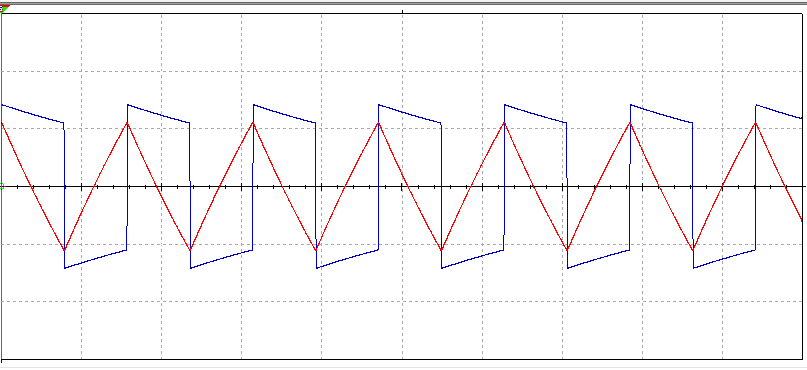
\includegraphics[width=\textwidth]{预习报告/4.png}
					\caption*{图8-13 仿真三角波波形}
				\end{minipage}
				\qquad
				\begin{minipage}{0.3\textwidth}
					\centering
					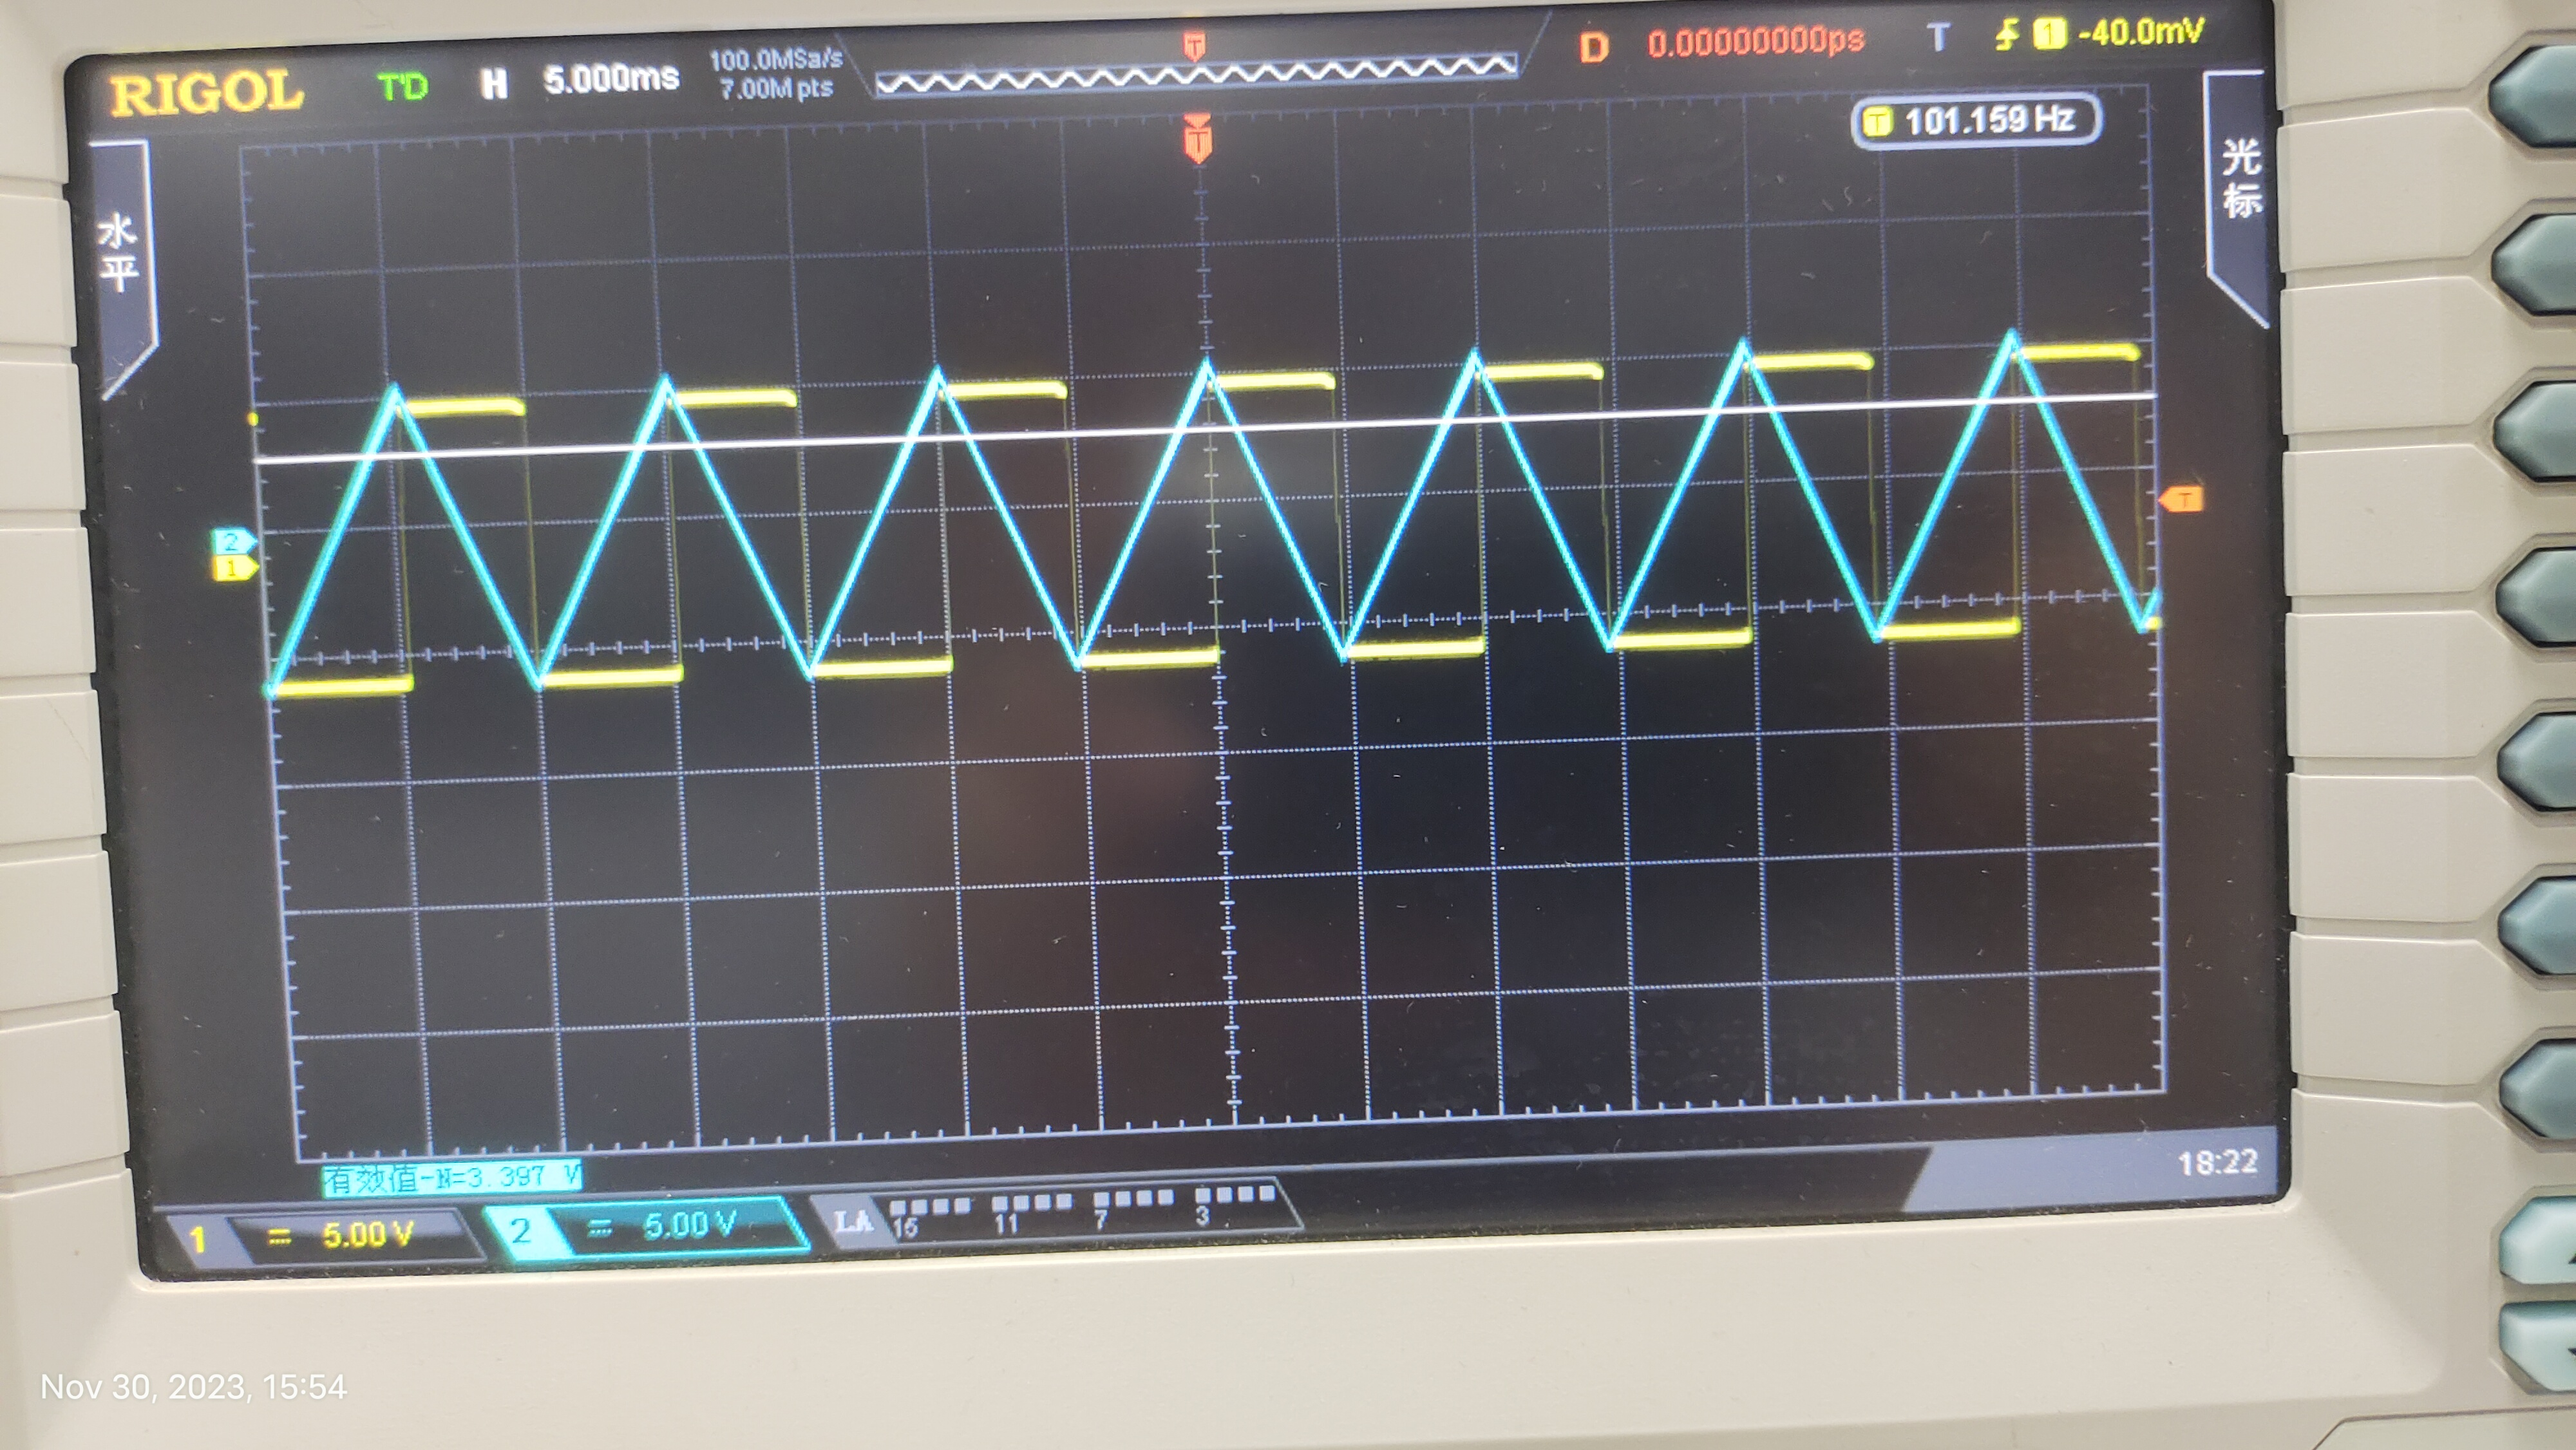
\includegraphics[width=\textwidth]{5.jpg}
					\caption*{图8-14 实验三角波波形}
				\end{minipage}
			\end{figure}
			\item 如何改变输出波形的频率?按预习方案分别实验并记录。\par 
			可以通过改变RP的阻值来改变波形频率\par 
			仿真波形如图8-15,实验波形如图8-16
			\begin{figure}
				\centering
				\begin{minipage}{0.3\textwidth}
					\centering
					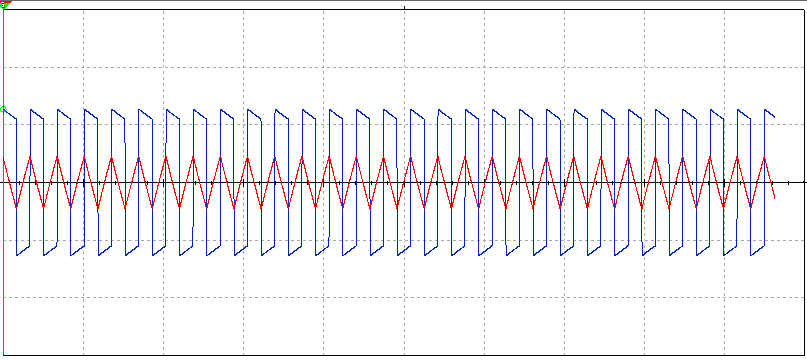
\includegraphics[width=\textwidth]{8.png}
					\caption*{仿真R=4$k\Omega$波形}
				\end{minipage}
				\qquad
				\begin{minipage}{0.3\textwidth}
					\centering
					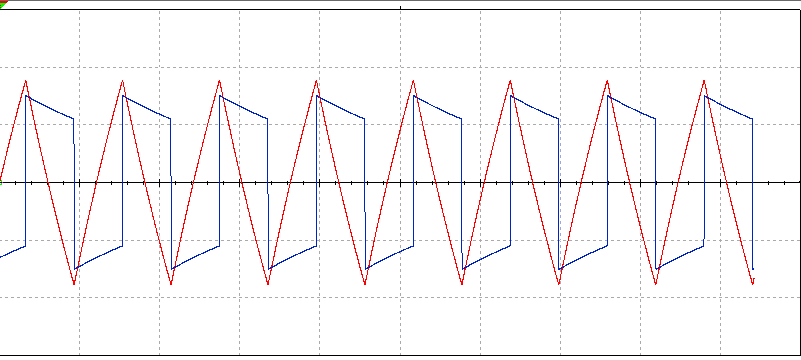
\includegraphics[width=\textwidth]{9.png}
					\caption*{仿真R=16$k\Omega$波形}
				\end{minipage}
				\caption*{图8-15 三角波仿真波形}
			\end{figure}
			\begin{figure}
				\centering
				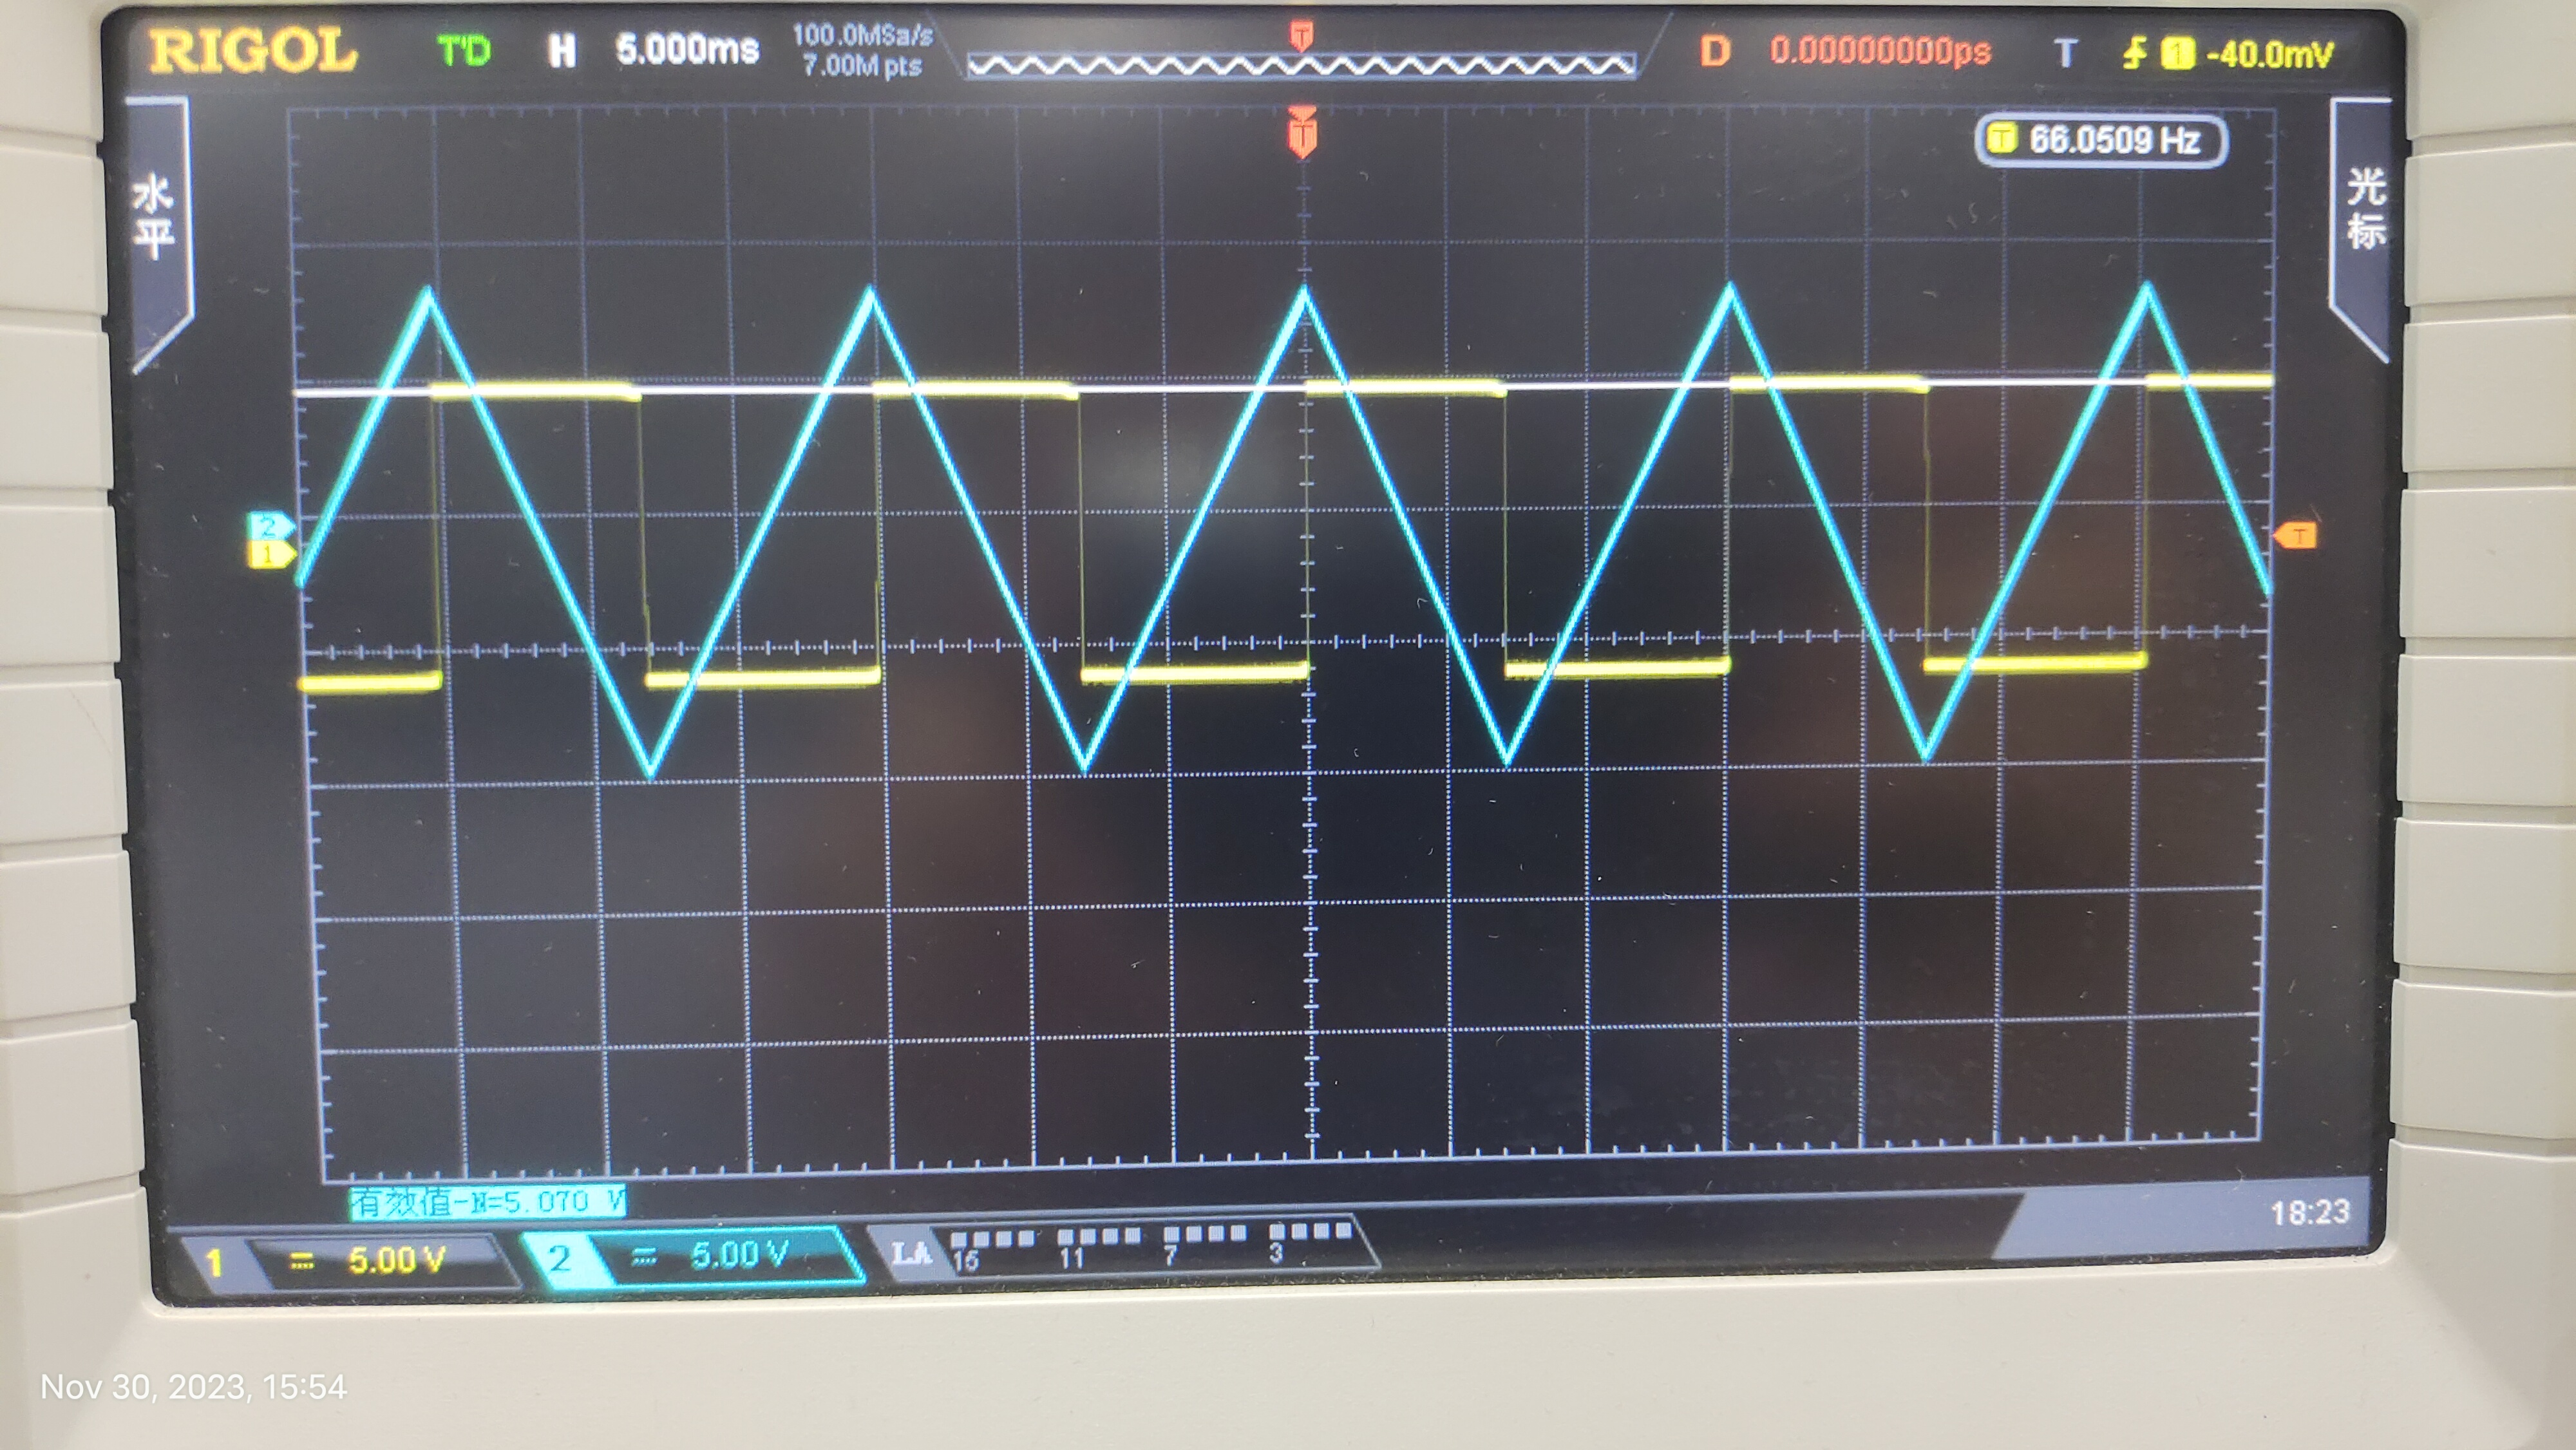
\includegraphics[width=0.4\textwidth]{6.jpg}
				\caption*{图8-16 增大R后的三角波实验波形}
			\end{figure}
		\end{enumerate}
		\item 锯齿波发生电路
		\begin{enumerate}
			\item 按图8-4 接线,观测Vo2 电路输出波形和频率。\par 
			仿真波形如图8-17,实验波形如图8-18
			\begin{figure}
				\centering
				\begin{minipage}{0.3\textwidth}
					\centering
					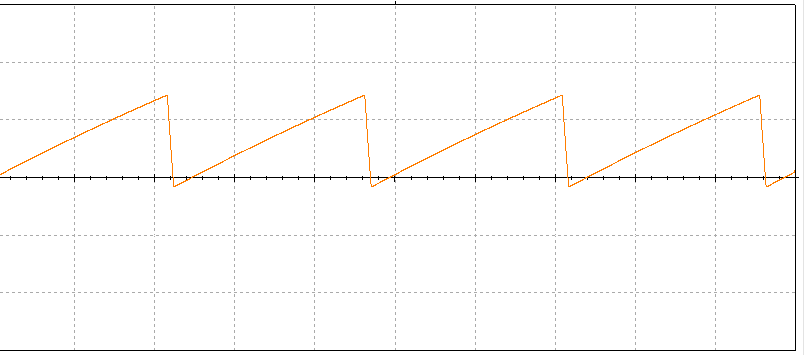
\includegraphics[width=\textwidth]{预习报告/5.png}
					\caption*{图8-17 仿真锯齿波波形}
				\end{minipage}
				\qquad
				\begin{minipage}{0.3\textwidth}
					\centering
					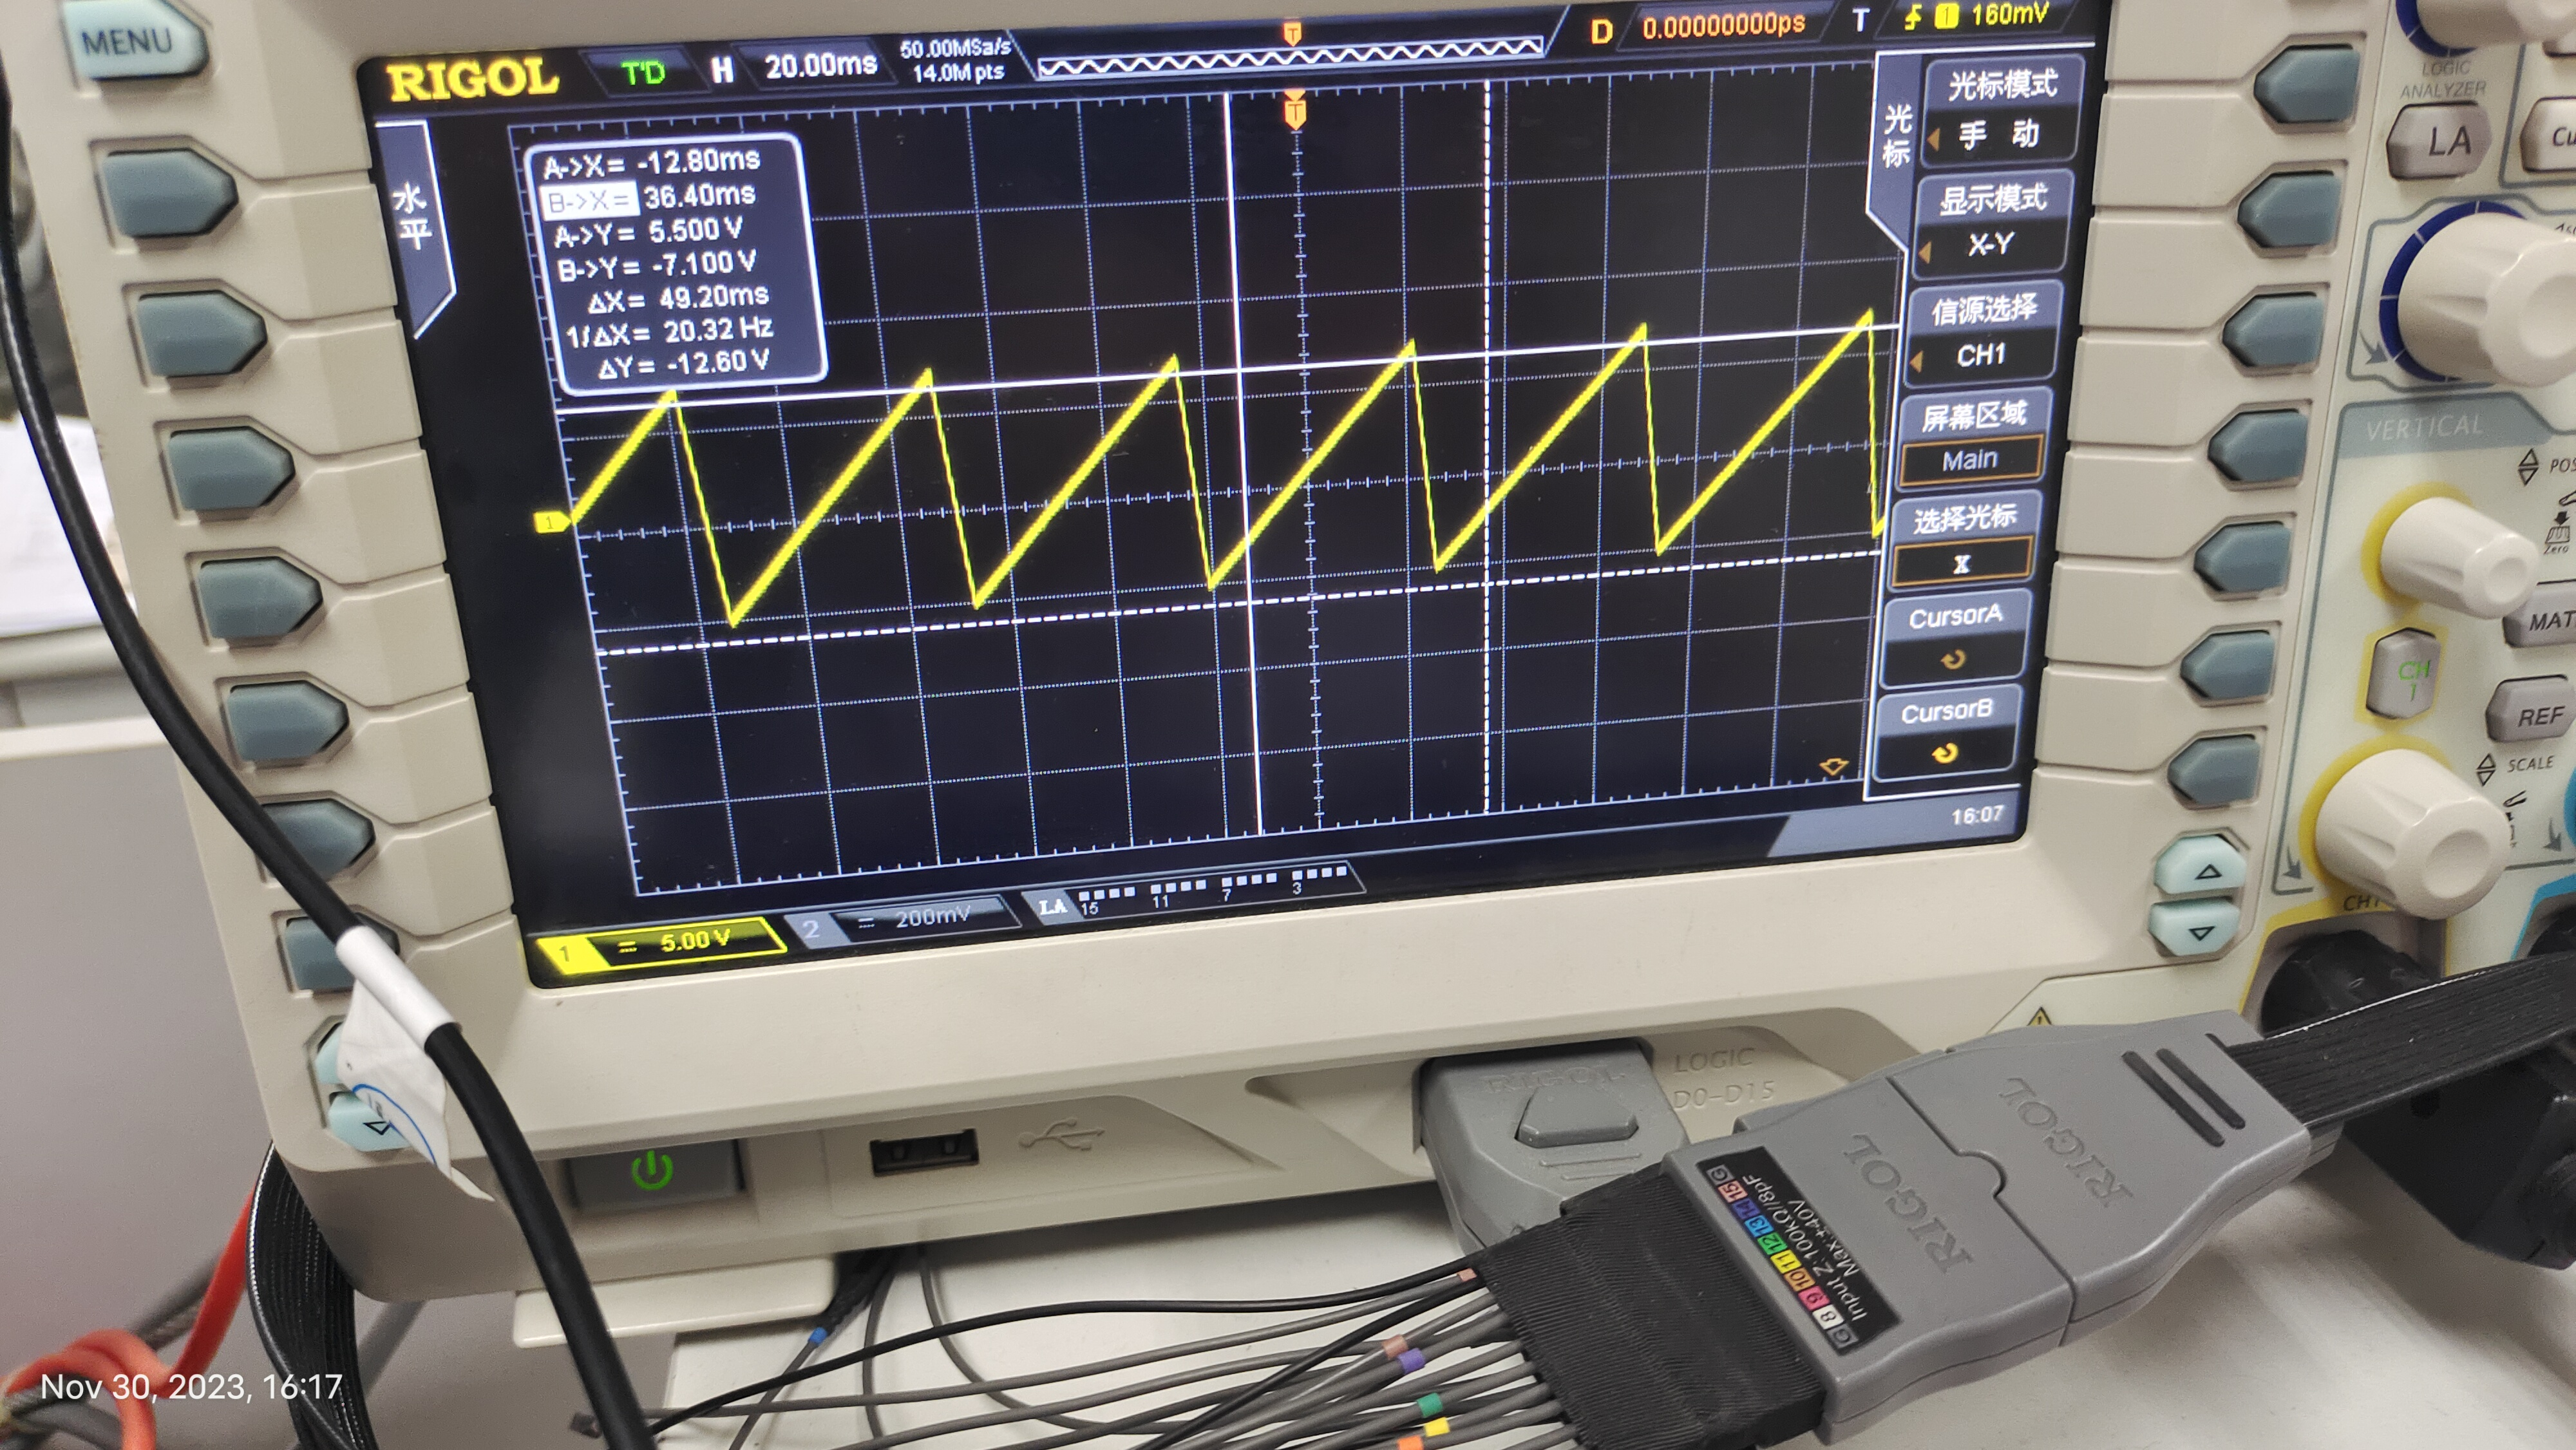
\includegraphics[width=\textwidth]{7.jpg}
					\caption*{图8-18 实验锯齿波波形}
				\end{minipage}
			\end{figure}
			\item 按预习时的方案改变锯齿波频率并测量变化范围。\par 
			可以通过改变滑动变阻器来改变频率变化范围,仿真结果为:24.57Hz--40.05Hz,实验结果为:20.23Hz-40.43Hz。
		\end{enumerate}
	\end{enumerate}
	\newpage
	\section*{四、实验器材}
	1、 实验箱 2、数字万用表 3、交流毫伏表 4、双踪示波器
	\section*{五、实验结果分析}
	\begin{enumerate}
		\item 对仿真和实验结果的分析
		\begin{enumerate}
			\item 在方波发生电路实验中,仿真和实验频率的波形接近,但是电压差别较大,后面经检查发现是限流
			电阻在实验过程中误接了51K$\Omega$i,导致电路偏小。
			\item 在方波发生电路中,实验波形相比于仿真波形的方波不平,主要原因是充放电时间过短导致
			\item 在占空比可调的矩形波发生电路中,实验频率和仿真频率相差较大,原因是实验时$R_{P2}$
			的阻值不等于仿真的阻值,又因为其阻值大小会影响频率,所以导致频率不一样,因此下次实验应该注意保持
			两者阻值相等,使仿真与实验具有可比性。
		\end{enumerate}
		\item 对波形发生电路特点的总结
		\begin{enumerate}
			\item 在许多情况下,波形发生电路不需要调零。因为电路的工作原理是正反馈,不会受到轻微的偏移或漂移的影响。
			\item 波形发生电路没有输入端,波形发生电路是基于内部元件和激励信号(电压源)来产生特定的波形,无需输入。
		\end{enumerate}
	\end{enumerate}
	\section*{六、预习报告}
	见附录
\end{document}